\documentclass[12pt,a4paper,twoside,openright,BCOR10mm,headsepline,titlepage,abstracton,chapterprefix,final]{scrreprt}

\usepackage{ae}
\usepackage[ngerman, english]{babel}
%\usepackage{SIunits}

\usepackage{amsmath}
\usepackage{amssymb}
\usepackage{amsfonts}
\usepackage{xcolor}
\usepackage{setspace}

% load hyperref as the last package to avoid redefinitions of e.g. footnotes after hyperref invokation

\RequirePackage{ifpdf}  % flag for pdf or dvi backend
\ifpdf
  \usepackage[pdftex]{graphicx}
  \usepackage[pdftitle={RTFM on Imaging Theory and Basics of Optical Raytracing},%
              pdfsubject={},%
              pdfauthor={M. Esslinger, J. Hartung, U. Lippmann},%
              pdfkeywords={},%
              bookmarks=true,%
%              colorlinks=true,%
              urlcolor=blue,%
              pdfpagelayout=TwoColumnRight,%
              pdfpagemode=UseNone,%
              pdfstartview=Fit,%
	      pdfpagelabels,
              pdftex]{hyperref}
\else
  \usepackage[dvips]{graphicx}
  \usepackage[colorlinks=false,dvips]{hyperref}
\fi
%\DeclareGraphicsRule{.jpg}{eps}{.jpg}{`convert #1 eps:-}

\usepackage{ae}
%\usepackage[ngerman, english]{babel}

%\usepackage{SIunits}
\newcommand\elementarycharge{\textrm{e}}
\newcommand\sccm{\textrm{sccm}}
\newcommand\mbar{\milli\textrm{bar}}


\usepackage{amsmath}
%\usepackage{amssymb}
\usepackage{setspace}

%\widowpenalty = 1000


\newcommand*{\doi}[1]{\href{http://dx.doi.org/\detokenize{#1}}{doi: \detokenize{#1}}}

\newcommand\Vector[1]{{\mathbf{#1}}}

\newcommand\vacuum{0}

\newcommand\location{r}
\newcommand\Location{\Vector{r}}


\newcommand\wavenumber{k}
\newcommand\vacuumWavenumber{\wavenumber_{\vacuum}}
\newcommand\Wavevector{\Vector{\wavenumber}}

\newcommand\Nabla{\Vector{\nabla}}
\newcommand\Laplace{\Delta}
\newcommand\timederivative[1]{\dot{{#1}}}
\newcommand\Tensor[1]{\hat{#1}}
\newcommand\conjugate[1]{\overline{#1}}
\newcommand\transpose[1]{#1^{T}}
\newcommand\Norm[1]{\left| #1 \right|}
\newcommand{\ket}[1]{\left\vert{#1}\right\rangle}
\newcommand{\bra}[1]{\left\langle{#1}\right\vert}
\newcommand{\braket}[2]{\left\langle{#1}\vert{#2}\right\rangle}
\newcommand{\bracket}[1]{\left\langle{#1}\right\rangle}

\newcommand{\scpm}[2]{(#1\,\cdot\,#2)}

\newcommand\Greenfunction{\Tensor{G}}

\newcommand\scalarEfield{E}
\newcommand\scalarBfield{B}
\newcommand\scalarHfield{H}
\newcommand\scalarDfield{D}
\newcommand\scalarTipfield{T}
\newcommand\scalarSamplefield{S}
\newcommand\scalarDipolarmoment{p}
\newcommand\Efield{\Vector{\scalarEfield}}
\newcommand\Bfield{\Vector{\scalarBfield}}
\newcommand\Hfield{\Vector{\scalarHfield}}
\newcommand\Dfield{\Vector{\scalarDfield}}
\newcommand\Dipolarmoment{\Vector{\scalarDipolarmoment}}

\newcommand\permeability{\Tensor{\mu}}
\newcommand\vacuumpermeability{\mu_{\vacuum}}
\newcommand\permittivity{\Tensor{\epsilon}}
\newcommand\generalPermittivity{\Tensor{\tilde\epsilon}}
\newcommand\vacuumpermittivity{\epsilon_{\vacuum}}
\newcommand\scalarpermittivity{\epsilon}
\newcommand\conductivity{\Tensor{\sigma}}
\newcommand\susceptibility{\Tensor{\chi}}
\newcommand\currentdensity{\Vector{j}}
\newcommand\Current{\Vector{I}}
\newcommand\chargedensity{\rho}
\newcommand\PoyntingVector{\Vector{S}}

\newcommand\ordi{\text{ord}}
\newcommand\eo{\text{eo}}

\newcommand{\timeavg}[1]{{\langle\,#1\,\rangle}}

\newcommand{\remark}[1]{{\color{red}$\blacksquare$}\footnote{{\color{red}#1}}}
\newcommand{\chk}[1]{\color{green}{$\checkmark$#1}}

\newcommand{\orderof}[1]{\mathcal{O}(#1)}


\begin{document}

\pagenumbering{roman}

\titlehead{ }
\subject{Pyrate -- Optical raytracing based on Python}
\title{Read This Fundamental Manual \\ on Imaging Theory and Basics of Optical Raytracing}
\author{M. Esslinger, J. Hartung, U. Lippmann}
\date{2014-2016}
\publishers{}
\maketitle

\onehalfspacing

\tableofcontents

\cleardoublepage

\pagenumbering{arabic}

\singlespacing

\section{No Warranty}
There is no warranty for the program, its manual, or goods designed using it to the extent permitted by applicable law. 
Except when otherwise stated in writing the copyright holders and/or other parties provide the program and its manual "as is" 
without warranty of any kind, either expressed or implied, 
including, but not limited to, the implied warranties of merchantability and fitness for a particular purpose. 
The entire risk as to the quality and performance of the program, its manual, or goods designed using it is with you. 
Should the program or its manual prove defective, you assume the cost of all necessary servicing, repair or correction.
In no event unless required by applicable law or agreed to in writing will any copyright holder, 
or any other party who may modify and/or redistribute the program or its manual as permitted by its license agreements, 
be liable to you for damages, including any general, special, incidental or consequential damages 
arising out of the use or inability to use the program 
(including but not limited to 
loss of data 
or data being rendered inaccurate 
or losses sustained by you or third parties 
or a failure of the program to operate with any other programs
or designs not conforming national law
or designs unfit for any particular purpose
or designs that are unsafe), 
even if such holder or other party has been advised of the possibility of such damages.

Using this program or its manual do not replace your own investigations and analyses using proper (that is, non-pyrate) sources. 
The copyright holders warn you that on-screen and/or printed versions of this manual may emit bosonic particles at speeds of 299792458\,m/s.

\chapter{Optics from Maxwell Equations}
\section{Maxwell Equations}
The content of this chapter is well known from textbooks \cite{Jackson, BornWolf}. Still, we repeat some of the equations to have a consistent 
nomenclature throughout this manual and the pyrate program as well as a gain in clarity which aproximations are made.
We start from the Maxwell equations in SI units
\begin{subequations}\label{eq:Maxwell}
\begin{eqnarray}
  \Nabla \Dfield &=& \chargedensity\,, 							\label{eq:MaxwellNablaD}\\
  \Nabla \times \Hfield -\timederivative{\Dfield} &=&  \currentdensity\,,  		\label{eq:MaxwellNablaCrossH} \\
  \Nabla \Bfield &=& 0\,,  									\label{eq:MaxwellNablaB} \\
  \Nabla \times \Efield + \timederivative{\Bfield} &=& 0\,,   					\label{eq:MaxwellNablaCrossE}
\end{eqnarray}
\end{subequations}
with the constitutive equations
\begin{subequations}\label{eq:Material}
\begin{eqnarray}
  \Dfield &=& \permittivity \Efield\,, 								\label{eq:ConstitutiveEpsilon}\\
  \Bfield &=& \permeability \Hfield\,, 								\label{eq:ConstitutiveMu}\\
  \currentdensity &=& \conductivity \Efield\,,						\label{eq:ConstitutiveSigma}
\end{eqnarray}
\end{subequations}
and the continuity equation, that follows directly from the Maxwell equations.
\begin{eqnarray}
  \Nabla \currentdensity + \timederivative{\chargedensity} &=& 0		\label{eq:continuity}
\end{eqnarray}
All quantities are real valued. $\permittivity$ is the  electric  permittivity, 
$\permeability$ the magnetic permeability, 
and $\conductivity$ the conductivity.
All material properties are described by unit bearing quantities, i.e., 
they are \emph{not} measured relative to the vacuum values $\vacuumpermittivity$ and $\vacuumpermeability$. 
We restrict ourselves to linear constitutive equations, that is, ($\permittivity$, $\permeability$ , $\conductivity$) do not depend on the field strength.
This limitation excludes treatment of effects like higher harmonic generation, frequency conversion, or wave mixing.
The Maxwell equations require media in which the constitutive bulk quantities can be assigned to all positions in space.
Single atoms, molecules or nanoscopic structures must be treated quantum-mechanically and are beyond the scope of this manual.

\section{Energy Conservation}
We assume the strictly monochromatic case $\Efield,\Dfield,\Hfield,\Bfield, \currentdensity \propto \sin(\omega t + \varphi_0)$ for electrodynamic scenarios only, $\omega \neq 0$.
We focus on the term
\begin{eqnarray}
   \Nabla ( \Efield \times \Hfield )
\end{eqnarray}
we apply the product rule for derivatives and rewrite the triple products, leading to
\begin{eqnarray}
   \Nabla ( \Efield \times \Hfield ) &=& \Hfield ( \Nabla \times \Efield ) - \Efield ( \Nabla \times \Hfield ) \\
   &=& - \Hfield \timederivative{\Bfield} - \Efield  \timederivative{\Dfield} - \Efield \currentdensity
\end{eqnarray}

We consider
\begin{eqnarray}
 \partial_t (\Efield \Dfield) &=& \Efield  \timederivative{\Dfield} +  \timederivative{\Efield} \Dfield \\
                              &=& \Efield ( \permittivity + \permittivity^T ) \timederivative{\Efield} 
\end{eqnarray}
In the monochromatic case, as assumed above, we can commutate $\partial_t$ and $\permittivity$.
We split up the permittivity into its symmetric and antisymmetric part $\permittivity =  \permittivity^S +  \permittivity^{AS}$ with
$(\permittivity^S)^T = \permittivity^S$ and $(\permittivity^{AS})^T = - \permittivity^{AS}$. 

\begin{eqnarray}
 \partial_t (\Efield \Dfield)                                                                  &=& 2 \Efield \permittivity^S \timederivative{\Efield} \\
 \frac{1}{2} \partial_t (\Efield \Dfield)+ \Efield \permittivity^{AS} \timederivative{\Efield} &=&   \Efield  \permittivity \timederivative{\Efield} \\
 \frac{1}{2} \partial_t (\Efield \Dfield)                                                      &=&   \Efield  \permittivity \timederivative{\Efield}
\end{eqnarray}

We derive an analogous equation for the magnetic field and insert both

\begin{eqnarray}
   \Nabla ( \Efield \times \Hfield ) + \frac{1}{2} \partial_t (\Hfield \Bfield) + \frac{1}{2} \partial_t (\Efield \Dfield) + \Efield \currentdensity &=& 0
\end{eqnarray}

leading to a continuity equation. 
We associate $\Efield \currentdensity$ with ohmic losses, that is, the volume density of energy losses from optical energy into other forms, for example heat.
Thus, the equation is a continuity equation of energy.
$\frac{1}{2} \Hfield \Bfield + \frac{1}{2} \Efield \Dfield$ is the energy density stored in a system, 
and $\Efield \times \Hfield$, which we call Poynting vector $\Vector{S}$, is the areal density of energy flow.
\begin{eqnarray}
 \Vector{S} &=& \Efield \times \Hfield
 \label{eq:definitionOfPoynting}
\end{eqnarray}
We discuss the Poynting vector in more detail in section \ref{sec:Poynting}, after introducing complex valued notation.

\section{Source-Free Maxwell Equations in Non-Magnetic Materials}
\label{sec:sourcefreemaxwell}
For ease of calculation, we introduce complex valued time harmonic dependence.
\begin{eqnarray}
 \Vector{F}(\Vector{r},t) &=& \Vector{F}_0(\Vector{r}) \exp(-i \omega t)
\end{eqnarray}
with $\Vector{F} \in \{ \Efield, \Dfield, \Hfield, \Bfield, \currentdensity \}$.
We associate the real part of $F$ with physically measureable quantities. 
Via the time harmonic factor $\exp(-i \omega t)$, the imaginary part of the fields will become real at other instances in time.
Complex valued amplitudes $\Vector{F}_0$ express magnitude and phase retardation of the fields.
All equations linear in $\Efield,\Dfield,\Hfield,\Bfield$ remain valid also for the newly introduced complex valued fields.
Care has to be taken with quadratic equations, 
containing terms like for example $\Efield \times \Hfield$, $\Hfield \Bfield$, or $\Efield \Dfield$,
as the square of a real number differs from that of a complex one -- e.g. it may become negative.

We assume all materials are non-magnetic at the optical frequency $\omega$, that is $\permeability(\omega) = \vacuumpermeability$. 
Effects like the Magneto-Optical Kerr Effect (MOKE) stem from the deflection of oscillating electrons in a static (DC) magnetic field and are typically modeled by off-diagonal elements in the permittivity tensor, not the permeability.
\begin{subequations}
\begin{eqnarray}
  \Nabla \Dfield &=& \chargedensity 					\\
  \Nabla \times \Efield &=& i \omega \vacuumpermeability \Hfield	\\
  \Nabla \Hfield &=& 0  					\\
  \Nabla \times \Hfield &=& - i \omega \Dfield + \currentdensity  		
\end{eqnarray}
\end{subequations}

The physically measurable fields are $\Efield$ and $\Bfield$, defined by forces on test charges. All other fields are fictional fields introduced in the Maxwell model for ease of calculation.
To obtain the so-called source-free Maxwell equations, we replace some of them by newly defined quantities.
We introduce a \emph{new} permittivity
\begin{eqnarray}
  \permittivity_{new} = \permittivity - \frac{\conductivity}{i \omega}
\end{eqnarray}
This newly defined permittivity is complex valued, where the imaginary part denotes electric conductivity and thus ohmic losses.
We introduce a corresponding \emph{new} $\Dfield$-field
\begin{eqnarray}
  \Dfield_{new} &=& \permittivity_{new} \Efield \\
  \Dfield &=& \Dfield_{new} + \frac{\conductivity}{i \omega} \Efield
\end{eqnarray}

In the Maxwell equations, we substitute the $\Dfield$-field by our newly defined field $\Dfield_{new}$.
With the conductivity equation \ref{eq:ConstitutiveSigma} and the continuity equation \ref{eq:continuity}, we find the so called source-free Maxwell equations
\begin{subequations}
\begin{eqnarray}
  \Nabla \Dfield_{new} &=& 0 					\label{eq:divDsourcefree}\\
  \Nabla \times \Efield &=& i \omega \vacuumpermeability \Hfield	\\
  \Nabla \Hfield &=& 0  					\\
  \Nabla \times \Hfield &=& - i \omega \Dfield_{new}  		
\end{eqnarray}
\end{subequations}
There are neither electric nor magnetic monopolar sources.
The equations are nearly symmetric in $\Dfield$ and $\Hfield$.
From now on, every time we write $\Dfield$, we mean the complex valued $\Dfield_{new}$ without explicitly writing the index \emph{new} (call us lazy, we don't care).
\begin{subequations}
\begin{eqnarray}
  \Nabla \Dfield &=& 0 					 	 \label{eq:sourcefreemaxwell_divD} \\
  \Nabla \times \Efield &=& i \omega \vacuumpermeability \Hfield \label{eq:sourcefreemaxwell_rotE}	\\
  \Nabla \Bfield &=& 0  					 \label{eq:sourcefreemaxwell_divB} \\
  \Nabla \times \Hfield &=& - i \omega \Dfield  		 \label{eq:sourcefreemaxwell_rotH}
\end{eqnarray}
\label{eq:sourcefreemaxwell}
\end{subequations}

\section{Poynting Vector}\label{sec:Poynting}
The Poynting vector is the a real density of energy flow. 
We want the Poynting vector to be real and stay numerically identical to the quantity derived above 
for the real valued Maxwell equations in equation \ref{eq:definitionOfPoynting}.

\begin{eqnarray}
 \Vector{S} &=& \Re \Efield \times \Re \Hfield \nonumber \\
            &=& \frac{1}{2} \Re ( \Efield \times \Hfield + \overline{\Efield} \times \Hfield ) \nonumber \\
            &=& \frac{1}{2} \Re ( \Efield_0 \times \Hfield_0 \exp(-2i\omega t) )
	      + \frac{1}{2} \Re ( \overline{\Efield}_0 \times \Hfield_0 ) \label{eq:SconjEH}\,,
\end{eqnarray}
for the decomposition $\Efield = \Efield_0 \exp(-i\omega t)$ and $\Hfield = \Hfield_0 \exp(-i\omega t)$.
The fast oscillation of the Poynting vector at $2 \omega$ is not directly measurable at optical frequencies, only its time average $\timeavg{\Vector{S}}$,
\begin{eqnarray}
 \timeavg{\Vector{S}}  &:=& \frac{\omega}{2\pi} \int_{0}^{2\pi / \omega} dt \, \Vector{S} \label{eq:timeaverageS}\,.
\end{eqnarray}
From \eqref{eq:SconjEH} and \eqref{eq:timeaverageS} we get
\begin{eqnarray}
  \timeavg{\Vector{S}}   &=& \underbrace{\left\langle \frac{1}{2} \Re ( \Efield_0 \times \Hfield_0 \exp(-2i\omega t) )\right\rangle}_{\approx0} + \frac{1}{2} \Re ( \overline{\Efield} \times \Hfield )\,.
\end{eqnarray}
We insert Maxwell equation \eqref{eq:sourcefreemaxwell_rotE} and obtain
\begin{eqnarray}
 \timeavg{\Vector{S}}   &=& \frac{1}{2} \Re \left( \overline{\Efield} \times \frac{\Nabla \times \Efield}{i \omega \vacuumpermeability} \right) \\
\end{eqnarray}
and via the Gra\ss mann identity 
\begin{eqnarray}
  \timeavg{\Vector{S}}_j &=&  \Re \frac{ \overline{\scalarEfield}_i \partial_j \scalarEfield_i - \overline{\scalarEfield}_j \partial_i \scalarEfield_i }{2 i \omega \vacuumpermeability}
\end{eqnarray}
The term $\partial_i \scalarEfield_i$ -- the divergence of the elctric field -- vanishes in isotropic, homogeneous media.
Assuming a plane wave expansion of $\Efield = \Vector{A} \exp(i \scpm{\Vector{k}}{\Location})$, we find
\begin{eqnarray}
  \partial_j E_i &=& i\,k_j E_i\,,
\end{eqnarray}
and
\begin{eqnarray}
 \timeavg{\Vector{S}}_j &=&  
    \frac{1}{2 \omega \vacuumpermeability}\Re( 
	\overline{\scalarEfield}_i \scalarEfield_i \delta_{j\ell}  
	- \overline{\scalarEfield}_j \scalarEfield_\ell 
      ) k_\ell\,.\label{eq:poyntingvector}
\end{eqnarray}
In general, the direction of the Poynting vector is the real projection of a weighted sum of the directions of $\Wavevector$ and $\Efield$.


\section{Plane Wave Solutions and Dispersion}
\subsection{The general anisotropic homgeneous case}
We consider a homogeneous material $\permittivity(\Location) = const.$ We apply the Nabla curl operatur on the Maxwell curl equation for the electric field
($\partial_i \partial_i =: \Delta$ the Laplacian). 
\begin{eqnarray}
  \Nabla \times ( \Nabla \times \Efield ) &=& \Nabla \times ( i \omega \vacuumpermeability \Hfield ) 
  \\
  \Delta \scalarEfield_j - \partial_j \partial_i \scalarEfield_i &=& - \omega^2 \vacuumpermeability \permittivity_{jk} \scalarEfield_{k} = -k_0^2 \permittivity_{jk} \scalarEfield_{k}
\end{eqnarray}
This is a differential equation with constant coefficients, so we use the ansatz
\begin{eqnarray}
 \Efield(\Location,\omega) &=& \Efield_0(\omega) \exp(i \Wavevector \Location)
\end{eqnarray}
where the $\Efield_0$ contains polarisation, electric field amplitude and harmonic time dependence.
With this monochromatic time dependence, $\permittivity_{ij}$ becomes a constant factor 
and we can replace $\partial_j \to i k_j$. We yield
\begin{align}
 A_{ij} E_{j\,0} &= 0 \label{eq:generalDispersionEigenEquationindex}\,.
\end{align}
with $A_{ij} = \left(-\Vector{k}^2 \delta_{ij} + k_i k_j + k_0^2 \permittivity_{ij} \right)$.
More explicit, it reads
\begin{eqnarray}
\begin{pmatrix}
 \wavenumber_y^2 + \wavenumber_z^2 - \omega^2 \vacuumpermeability \scalarpermittivity_{xx} 
 &
 - \wavenumber_x \wavenumber_y - \omega^2 \vacuumpermeability \scalarpermittivity_{xy}
 &
 - \wavenumber_x \wavenumber_z - \omega^2 \vacuumpermeability \scalarpermittivity_{xz}
 \\
 - \wavenumber_x \wavenumber_y - \omega^2 \vacuumpermeability \scalarpermittivity_{yx}
 &
 \wavenumber_x^2 + \wavenumber_z^2 - \omega^2 \vacuumpermeability \scalarpermittivity_{yy} 
 &
 - \wavenumber_y \wavenumber_z - \omega^2 \vacuumpermeability \scalarpermittivity_{yz}
 \\
 - \wavenumber_x \wavenumber_z - \omega^2 \vacuumpermeability \scalarpermittivity_{zx}
 &
 - \wavenumber_y \wavenumber_z - \omega^2 \vacuumpermeability \scalarpermittivity_{zy}
 &
 \wavenumber_x^2 + \wavenumber_y^2 - \omega^2 \vacuumpermeability \scalarpermittivity_{zz}  
\end{pmatrix}
\Efield_0
&=& 0 \label{eq:generalDispersionEigenEquation}
\end{eqnarray}
Nontrivial solutions can be found if the determinant of $\hat{A}$ is zero.
In general, each solution $\Wavevector$ is associated with a certain eigenvector direction $\Efield_0$,
that is, a propagation wavector is only valid for a certain polarisation.
We use the identity
\begin{align}
 \det A &= \frac{1}{6} ((\text{tr} A)^3 - 3 (\text{tr} A) \text{tr}(A^2) + 2 \text{tr}(A^3))\,,
\end{align}
We also factor out a permittivity of the vacuum from the permittivity tensor 
$\permittivity_{ij} \to  \vacuumpermittivity \permittivity_{ij}$ and introduce the ``vacuum wave number''
$k_0 := \frac{2\pi}{\lambda_0} = \frac{\omega}{c} = \omega \sqrt{\vacuumpermeability  \vacuumpermittivity}$.
and rewrite the determinant
\begin{align}
 \det \hat{A}(\Vector{k}) 
 &= k_0^2 \left(\frac{1}{6} \alpha k_0^4 +  (-\beta \text{tr}\permittivity + \gamma) k_0^2 + \Vector{k}^2 \beta \right)=0\,,\label{eq:determinantinvariant}
\end{align}
where $\alpha = (\text{tr}\permittivity)^3 - 3 (\text{tr}\permittivity) \text{tr}(\permittivity^2) + 2 \text{tr}(\permittivity^3)$,
$\beta = \permittivity_{ij} k_i k_j$, $\gamma = k_i \permittivity_{i\ell} \permittivity_{\ell j} k_j$. For given $\omega$ this is an equation of fourth order
for some inplane component of $\Vector{k}$. The first part in the determinant does not depend on $\Vector{k}$. Therefore the differentiation with respect to
$\Vector{k}$ gives only two terms.
\begin{align}
 \frac{\partial D}{\partial k_j} &= k_0^2 
\left[
k_0^2
\left(
  \permittivity_{ji} (-(\text{tr}\permittivity) k_i + \permittivity_{i\ell} k_\ell)
+ \permittivity_{ij} (-(\text{tr}\permittivity) k_i + \permittivity_{\ell i} k_\ell)
\right)
+ (\permittivity_{\ell j} + \permittivity_{j \ell}) \Vector{k}^2 k_\ell + 2 \beta k_j
\right]
\end{align}

\subsection{Uniaxial anisotropic, homogeneous media}
Uniaxial anisotropic media are media with one axis, along which the permittivity takes an extraordinary value, 
and a degenerate permittivity along the other two directions in space.
The direction along which the extraordinary permittivity occurs is often called \emph{optical axis}. 
In this manual, we use the term \emph{extraordinary direction} $\Vector{e}_{eo}$, to avoid confusion with the symmetry axis of radially symmetric lens systems in technical optics.

Often, these materials have a crystalline structure with a degenerate rectangular or hexagonal plane in the unit cell, 
and a strongly deviating unit vector in the orthogonal direction. 

Without loss of generality, we choose our coordinate system so that the extraordinary direction is aligned with the cartesian $z$ axis.
\begin{eqnarray}
 \permittivity &=&
 \begin{pmatrix}
  \scalarpermittivity_{\ordi}  & 0 & 0 \\
  0 & \scalarpermittivity_{\ordi}  & 0 \\
  0 & 0 & \scalarpermittivity_{\eo}   \\
 \end{pmatrix}
\end{eqnarray}

We further rotate the coordinate system in the degenerate $xy$ plane so that $\wavenumber_y = 0$.
The eigenvalue equation \ref{eq:generalDispersionEigenEquation} simplifies to

\begin{eqnarray}
\begin{pmatrix}
 \wavenumber_z^2 - \omega^2 \vacuumpermeability \scalarpermittivity_{\ordi} 
 &
 0
 &
 - \wavenumber_x \wavenumber_z 
 \\
 0
 &
 \wavenumber_x^2 + \wavenumber_z^2 - \omega^2 \vacuumpermeability \scalarpermittivity_{\ordi} 
 &
 0 
 \\
 - \wavenumber_x \wavenumber_z 
 &
 0 
 &
 \wavenumber_x^2 - \omega^2 \vacuumpermeability \scalarpermittivity_{\eo}  
\end{pmatrix}
\Efield_0
&=& 0
\end{eqnarray}

The equation system splits up into a coupled system of $\scalarEfield_x$ and $\scalarEfield_z$ , and an independent equation for $\scalarEfield_y$

\begin{subequations}
\begin{align}
\begin{pmatrix}
 \wavenumber_z^2 - \omega^2 \vacuumpermeability \scalarpermittivity_{\ordi} 
 &
 - \wavenumber_x \wavenumber_z 
 \\
 - \wavenumber_x \wavenumber_z 
 &
 \wavenumber_x^2 - \omega^2 \vacuumpermeability \scalarpermittivity_{\eo}  
\end{pmatrix} 
\begin{pmatrix}
 \scalarEfield_x 
 \\
 \scalarEfield_z
\end{pmatrix}
&= 0
\\
\begin{pmatrix} \wavenumber_x^2 + \wavenumber_z^2 - \omega^2 \vacuumpermeability \scalarpermittivity_{\ordi} \end{pmatrix} \scalarEfield_y &= 0\,.
\end{align}
\end{subequations}

We call the solutions of the equation for $\scalarEfield_y$ ordinary mode, and of the coupled system extraordinary mode.
We find the following eigenvalues and eigenvectors:
\subsubsection{Ordinary mode (ord)}

If the wavevector fulfills the equation
\begin{eqnarray}
  \wavenumber_x^2 + \wavenumber_z^2 - \omega^2 \vacuumpermeability \scalarpermittivity_{\ordi} &=& 0 
\end{eqnarray}
We have a nontrivial solution for the electric field in $y$-direction.

\begin{eqnarray}
 \Wavevector^2 &=& \omega^2 \vacuumpermeability \scalarpermittivity_{\ordi} 
 \\
 \Efield &\propto& \Vector{e}_{eo} \times \Wavevector
\end{eqnarray}
For the ordinary mode, $\Efield$ is orthogonal on both $\Wavevector$ and the extraordinary direction.
The Poynting vector points in the direction of the real part of $\Wavevector$,
\begin{eqnarray}
 \timeavg{\Vector{S}}_\ordi = \frac{ |\scalarEfield|^2 }{ 2\omega\vacuumpermeability } \Re \Wavevector\,.\label{eq:Suniaxialordi}
\end{eqnarray}


\subsubsection{Extraordinary mode (eo)}
\begin{eqnarray}
  \frac{\wavenumber_{x}^2 }{\scalarpermittivity_{\eo} } + \frac{\wavenumber_{z}^2 }{\scalarpermittivity_{\ordi} } &=& \omega^2 \vacuumpermeability 
  \label{eq:uniaxialAnisotropicDispersion}
  \\
  \scalarEfield_x \scalarpermittivity_{\ordi} \wavenumber_x &=& -  \scalarEfield_z \scalarpermittivity_{\eo} \wavenumber_z \label{eq:divDuniaxial}
\end{eqnarray}

The Poynting vector from \eqref{eq:poyntingvector} is given by
\begin{eqnarray}
 \timeavg{\Vector{S}}_j &=&  \Re\frac{1}{2 \omega \vacuumpermeability}\left[ (|\scalarEfield_x|^2 + |\scalarEfield_z|^2) \delta_{j\ell}  - \overline{\scalarEfield}_j \scalarEfield_\ell \right] k_\ell\,.
\end{eqnarray}
With \eqref{eq:divDuniaxial} we may derive an expression for the divergence appearing in the second term by inserting an ``intelligent zero''
\begin{eqnarray}
 0 &=& \scalarEfield_x \wavenumber_x + \frac{\scalarpermittivity_{\ordi}}{\scalarpermittivity_\eo} \scalarEfield_z \wavenumber_z\,,\nonumber\\
&\Rightarrow& \scalarEfield_x \wavenumber_x + \scalarEfield_z \wavenumber_z = \scalarEfield_z \wavenumber_z \left(1 - \frac{\scalarpermittivity_{\ordi}}{\scalarpermittivity_\eo}\right)\,. \label{eq:divEviolation}
\end{eqnarray}
Therefore the Poynting vector consists of two terms like in the general case
\begin{eqnarray}
  \timeavg{\Vector{S}} = \frac{ 1 }{ 2\omega\vacuumpermeability } \Re 
  \left[
      (|\scalarEfield_x|^2 + |\scalarEfield_z|^2)\Wavevector
      - \left(1 - \frac{\scalarpermittivity_{\ordi}}{\scalarpermittivity_\eo}\right)\scalarEfield_z \wavenumber_z \overline{\Efield}
  \right]\,.\label{eq:Suniaxialeo}
\end{eqnarray}
For general coordinate systems, where the extraordinary axis points in the direction $\Vector{e}_{eo}$, 
we replace $E_z \rightarrow E_i e_{\eo, i}$ and find
\begin{eqnarray}
  \timeavg{S}_j = \frac{ 1 }{ 2\omega\vacuumpermeability } \Re 
  \left[
      \scalarEfield_i \overline{\scalarEfield}_i \wavenumber_j
      + \left(\frac{\scalarpermittivity_{\ordi}}{\scalarpermittivity_\eo} - 1\right)
        (\scalarEfield_m e_{\eo,m}) (\wavenumber_n e_{\eo,n}) \overline{\scalarEfield}_j
  \right]
\end{eqnarray}


\subsection{Isotropic media}

We use the result for uniaxial anisotropic materials and insert the same value for both ordinary and extraordinary permittivity $\scalarpermittivity_{\ordi} = \scalarpermittivity_{\eo} = \scalarpermittivity$.
This results in a degenerate solution for both polarisations,
\begin{eqnarray}
 \Wavevector^2 &=& \omega^2 \vacuumpermeability \scalarpermittivity\,, \\
 \scpm{\Wavevector}{\Efield} &=& 0\,.
\end{eqnarray}
where $\Wavevector^2$ is not the absolute square, but the scalar product of the wavevector with itself.
For plane waves in isotropic media, the Poynting vector becomes 
\begin{eqnarray}
 \timeavg{\Vector{S}}_\text{iso} = \frac{ |\Efield|^2 }{ 2\omega\vacuumpermeability } \Re \Wavevector
\end{eqnarray}

We introduce the refractive index $n$ as
\begin{eqnarray}
 \Wavevector^2 &=& k_0^2 n^2 \\
 n &=& \pm \sqrt{ \frac{\scalarpermittivity}{\vacuumpermittivity} }
\end{eqnarray}
In general, there are two roots. 
The choice of the root does not change anything in optics based on the Maxwell equations, as the permittivity is the only physically relevant quantity.




\section{Boundary Conditions}
Considering two media $\permittivity_1$ and $\permittivity_2$, we find the following conditions fulfilled on the boundary in both media \cite{Jackson}:
\begin{subequations}
\begin{eqnarray}
 ( \Dfield_2 - \Dfield_1 ) \Vector{n} &=& 0 \\
 ( \Bfield_2 - \Bfield_1 ) \Vector{n} &=& 0 \\
 \Vector{n} \times ( \Efield_2 - \Efield_1 ) &=& 0 \\
 \Vector{n} \times ( \Hfield_2 - \Hfield_1 ) &=& 0 
\end{eqnarray}
\label{eq:boundary_conditions} 
\end{subequations}
where $\Vector{n}$ is the surface normal unit vector.
These relations hold for a step-interface between two homogeneous media. 
In mesoscopically inhomogenous media like  diffractive optical elements and metamaterials, 
the boundary conditions hold at each interface between homogeneous materials of the mesoscopic sub-structure.


\section{Reflection and Refraction of Plane Waves at Planar Surfaces}

\subsection{Derivation}
We consider a plane wave incident on a planar boundary between two homogeneous materials.
The incident plane wave projects a grating on the boundary plane. 
The fields $\Dfield_{in}$ and $\Efield_{in}$ on the boundary in medium $\permittivity_1$ are modulated with the in-plane component of the wavevector. 
\begin{eqnarray}
 \Dfield_{in}, \Efield_{in} &\propto& \exp( i \Wavevector_{in\parallel} \Location)|_{boundary} \\
 \Wavevector_{in\perp} &=& ( \Wavevector_{in} \Vector{n} ) \Vector{n} \\
 \Wavevector_{in\parallel} &=& \Wavevector_{in} - \Wavevector_{in\perp}
\end{eqnarray}
where $\Vector{n}$ is the surface normal unit vector.
From the boundary conditions \ref{eq:boundary_conditions} we conclude that with $\Dfield_{in}$ and $\Efield_{in}$, 
all reflected or refracted modes $M$ are to be modulated by the same in-plane wavevector component.
\begin{eqnarray}
  \Dfield_{M}, \Efield_{M} &\propto& \exp( i \Wavevector_{M\parallel} \Location)|_{boundary} \\
  \Wavevector_{M\parallel} &=& \Wavevector_{in\parallel}
\end{eqnarray}
The in-plane wave vector component is conserved.
To find the reflected and refracted modes, 
we fix the in-plane wavevector component and search for solutions of the material dispersion
(equation \ref{eq:generalDispersionEigenEquation}).
In general, the dispersion is quartic and allows for 4 solutions in each medium.
\begin{figure}
  \centering
   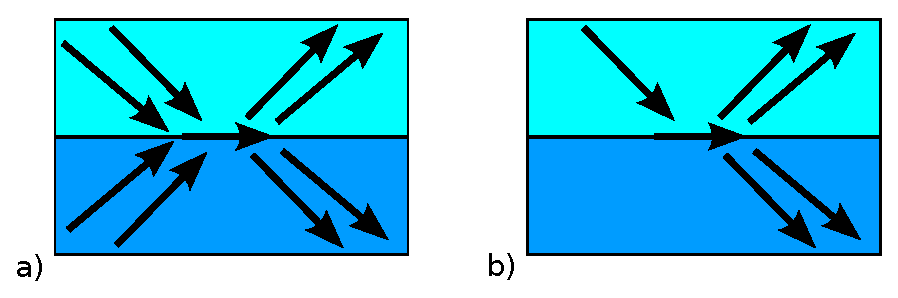
\includegraphics[width=0.5\columnwidth]{boundary_wavevectors}
  \caption{a) Wavevectors with the same in-plane component.
           b) Scenario of a single incident plane wave.}
  \label{fig:boundary_wavevectors}
\end{figure}
In each medium, there are 2 solutions transporting energy towards the boundary, 
and 2 solutions transporting energy from it (see figure \ref{fig:boundary_wavevectors}).
The modes can be distinguished by analyzing the direction of the Poynting vector relative to the surface normal,
$\Vector{S}\cdot\Vector{n}>0$ or $\Vector{S}\cdot\Vector{n}<0$.
In the scenario we consider, we have a single incident plane wave from medium $1$, 
and we discard the 3 remaining solutions transporting energy towards the boundary.
This leaves 5 modes: One incident plane wave splits up into 2 reflected modes and 2 refracted modes.
We consider the electric fields $\Efield_{1,2}$ on both sides of the boundary
\begin{subequations}
\begin{eqnarray}
 \Efield_1(\Location) &=& \Efield_{in,0} \exp(i \Wavevector_{in} \Location) + \Efield_{r1,0} \exp(i \Wavevector_{r1} \Location) + \Efield_{r2,0} \exp(i \Wavevector_{r2} \Location)  \\
 \Efield_2(\Location) &=& \Efield_{t1,0} \exp(i \Wavevector_{t1} \Location) + \Efield_{t2,0} \exp(i \Wavevector_{t2} \Location)
\end{eqnarray}
\label{eq:modes_on_boundary} 
\end{subequations}

Each term on the right hand side stands for a mode, represented by its amplitude $\Efield_{0}$ and wavevector $\Wavevector$.
We consider the incident mode $\Wavevector_{in}$, 
the two reflected modes $\Wavevector_{r1,2}$,
and the two refracted or transmitted modes $\Wavevector_{t1,2}$.
For isotropic media 1, the modes $\Wavevector_{r1,2}$ degenerate. 
The same holds for $\Wavevector_{t1,2}$ in isotropic media 2.

\subsection{The Law of Refraction}
Our formulation of the law of refraction and the law of reflection is
\begin{eqnarray}
 \Wavevector_{M} &=& \Wavevector_{in\parallel} + \xi_M \Vector{n}\,.\label{eq:xieqn}
\end{eqnarray}
The wavevectors of each mode $\Wavevector_M$ consist of the conserved in-plane component $\wavenumber_{in\parallel}$ and the out-of-plane component $\xi_M$. 
Solving the material dispersion $\xi$, we find the directions of all refracted and reflected modes.
Compared to the law of Snellius, this formulation bears the following advantages:
\begin{itemize}
 \item It does not require the calculation of angles in 3D space, only scalar products.
 \item The incident wavevector can be modelled as a property of the ray. When calculating the refracted wavevector, 
       the dispersion relation in material $\permittivity_1$ is not required.
       This allows to isolate methods in object-oriented programming and a modular design.
 \item It is not required to implement a different law of refraction for each \emph{pair} of material classes interfacing 
       (isotropic, uniaxial anisotropic, biaxial anisotropic, magnetooptic, ...),
       where the number of implementations increases quadratically with the number of material classes.
       Instead, the effort of solving the material dispersion increases linearly.
 \item We can calculate with complex valued permittivities, that is, lossy materials.
       The law of Snellius coincides with the Maxwell equations for real valued positive refractive indices only.
 \item We can handle anisotropic materials.
\end{itemize}
The formulation does not actually solve the problem of refraction, but forwards it to the problem of finding a solution $\xi$ of the material dispersion. 
This calculation can, for certain types of anisotropic materials, be complicated.

\subsubsection{isotropic media}
\begin{align}
 \xi = \sqrt{k_0^2 \epsilon_2 - \Wavevector_{1\,\parallel}^2}
\end{align}

where $\Wavevector_{1\,\parallel}^2$ is the scalar product of the in-plane wavevector projection with itself.
It is not the absolute of the wavevector component and may be complex valued for lossy materials.


\subsubsection{uniaxial anisotropic}
The ordinary mode behaves like the isotropic solution.
The material dispersion of the extraordinary mode, equation \ref{eq:uniaxialAnisotropicDispersion}, is

\begin{eqnarray}
 \Wavevector^2 \scalarpermittivity_{\ordi} 
 + \wavenumber_{z}^2 (\scalarpermittivity_{\eo} - \scalarpermittivity_{\ordi})
 &=& \omega^2 \vacuumpermeability \scalarpermittivity_{\ordi} \scalarpermittivity_{\eo} 
 \\
 (\Wavevector_{1\,\parallel}^2 + \xi^2) \scalarpermittivity_{\ordi} 
 + (\Wavevector_{1\,\parallel} \Vector{e}_{\eo} + \xi \Vector{n}\Vector{e}_{\eo})^2 (\scalarpermittivity_{\eo} - \scalarpermittivity_{\ordi})
 &=& \omega^2 \vacuumpermeability \scalarpermittivity_{\ordi} \scalarpermittivity_{\eo}  
\end{eqnarray}
This is a quadratic equation in $\xi$.
\begin{eqnarray}
 c_2 \xi^2 + c_1 \xi + c_0 &=& 0
 \\
 c_2 &=& \scalarpermittivity_{\ordi} + (\scalarpermittivity_{\eo} - \scalarpermittivity_{\ordi}) (\Vector{n}\Vector{e}_{\eo})^2
 \nonumber 
 \\
 c_1 &=& 2 (\scalarpermittivity_{\eo} - \scalarpermittivity_{\ordi}) (\Wavevector_{1\,\parallel} \Vector{e}_{\eo}) (\Vector{n}\Vector{e}_{\eo})
 \nonumber 
 \\
 c_0 &=& \Wavevector_{1\,\parallel}^2 \scalarpermittivity_{\ordi} + (\scalarpermittivity_{\eo} - \scalarpermittivity_{\ordi}) (\Wavevector_{1\,\parallel} \Vector{e}_{\eo})^2 
       - \omega^2 \vacuumpermeability \scalarpermittivity_{\ordi} \scalarpermittivity_{\eo} 
 \nonumber
\end{eqnarray}

\subsubsection{general anisotropic}
We start from the general dispersion relation \eqref{eq:determinantinvariant} and decompose $\Wavevector$ into in-plane and off-plane part
$\Wavevector = \Wavevector_\parallel + \xi \Vector{n}$.
We divide the equation by $\omega^2 \vacuumpermeability$ and yield
\begin{align}
0 &= c_4 \xi ^4 + c_3 \xi ^3 + c_2 \xi ^2 + c_1 \xi + c_0
\end{align}
with
\begin{align}
 c_4 &= \permittivity_{ij} n_i n_j \\
 c_3 &= \left[a_8+a_9\right] \\
 c_2 &= \left[\tilde{\omega} ^2 (a_{13}-a_1 c_4)+ a_4 c_4+a_5\right] \\
 c_1 &= \left[\tilde{\omega}^2 (-a_1 c_3 + a_{11}+a_{12})+a_4 c_3\right] \\
 c_0 &= \frac{1}{6} \tilde{\omega} ^4 \left(a_1^3-3 a_1 a_2+2 a_3\right) +\tilde{\omega}^2 (a_6-a_1 a_5)+a_4 a_5
\end{align}
with
\newcommand{\kpa}[1]{{k_{\parallel\,#1}}}
\begin{subequations}
\begin{align}
\tilde{\omega} &= \omega \sqrt{\mu_0}\\
 a_1 &= \permittivity_{ii} \\
 a_2 &= \permittivity_{ij}\permittivity_{ji} \\ 
 a_3 &= \permittivity_{ij}\permittivity_{jk}\permittivity_{ki} \\
 a_4 &= \kpa{i}\kpa{i} \\
 a_5 &= \permittivity_{ij} \kpa{i} \kpa{j} \\
 a_6 &= \permittivity_{ij} \permittivity_{jk} \kpa{i}\kpa{k} \\
 a_8 &= \permittivity_{ij} \kpa{j} n_i \\
 a_9 &= \permittivity_{ij} \kpa{i} n_j \\
 a_{11} &= \permittivity_{ij} \permittivity_{jk} \kpa{k} n_i \\
 a_{12} &= \permittivity_{ij} \permittivity_{jk} \kpa{i} n_k \\
 a_{13} &= \permittivity_{ij} \permittivity_{jk} n_i n_k 
\end{align}
\end{subequations}







\subsection{Fresnel Coefficients}
Assume we solved the material dispersion and found the wavevectors of all modes as well as their corresponding eigen-polarizations
\begin{subequations}
\begin{eqnarray}
(\Wavevector_{in}, \Wavevector_{r1}, \Wavevector_{r2}, \Wavevector_{t1}, \Wavevector_{t2}) \\
(\Vector{e}_{in}, \Vector{e}_{r1}, \Vector{e}_{r2}, \Vector{e}_{t1}, \Vector{e}_{t2})
\end{eqnarray}
\end{subequations}
The field of each mode $M \in \{ r1, r2, t1, t2 \}$
\begin{eqnarray}
\Efield_{M} &=& E_{M,0} \Vector{e}_{M} \exp{i \Wavevector_M \Location}
\end{eqnarray}
depends on the scalar amplitude $E_{M,0}$, containing mode strength and retardation.
We combine the boundary conditions \ref{eq:boundary_conditions} and \ref{eq:modes_on_boundary} with this ansatz and yield an equation system
\begingroup \small
\begin{subequations}
\begin{align}
   - ( \permittivity_1 \Vector{e}_{r1}) \Vector{n} E_{r1,0} &-& ( \permittivity_1 \Vector{e}_{r2}) \Vector{n} E_{r2,0} &+& ( \permittivity_2 \Vector{e}_{t1} ) \Vector{n} E_{t1,0} &+& ( \permittivity_2 \Vector{e}_{t2} ) \Vector{n} E_{t2,0} &=& \Dfield_{in} \Vector{n} \label{eq:fresneldn}\\
   - ( \Vector{e}_{r1} \times \Vector{n} )         E_{r1,0} &-& ( \Vector{e}_{r2} \times \Vector{n} )         E_{r2,0} &+& ( \Vector{e}_{t1} \times \Vector{n} )          E_{t1,0} &+& ( \Vector{e}_{t2} \times \Vector{n} )          E_{t2,0} &=& \Efield_{in} \times \Vector{n} \label{eq:fresnelEcrossn} \\
   - ( \Wavevector_{r1} \times \Vector{e}_{r1} )   E_{r1,0} &-& ( \Wavevector_{r2} \times \Vector{e}_{r2} )   E_{r2,0} &+& ( \Wavevector_{t1} \times \Vector{e}_{t1} )    E_{t1,0} &+& ( \Wavevector_{t2} \times \Vector{e}_{t2} )    E_{t2,0} &=& \Wavevector_{in} \times \Efield_{in} \label{eq:fresnelkE}
\end{align}
\end{subequations}
\endgroup
All prefactors $\permittivity, \Vector{e}, \Wavevector, \Vector{n}$ are known, 
as well as the incident wave properties on the right hand side of the equations.
Our goal is to solve this linear equation system for the amplitudes $E_{M,0}$.
We have 7 scalar equations, and only 4 unknowns.
The system, however, is not of full rank.
Before solving the system, we need to reduce the number of equations.

First, we split up the mode label $M$ into two indices $\alpha=1,2$ and $\beta=r,t$.
This allows us to abbreviate the equation system to
\begin{subequations}
  \begin{align}
    \sum_{\alpha=1,2\;\beta=r,t} \varsigma_\beta (\permittivity_\alpha \Vector{e}_{\beta\alpha})\Vector{n} E_{\beta\alpha,0} &= \Dfield_{in} \Vector{n}                   \label{eq:FresnelSystemEq1} \\
    \sum_{\alpha=1,2\;\beta=r,t} \varsigma_\beta (\Vector{e}_{\beta\alpha} \times \Vector{n} ) E_{\beta\alpha,0} &= \Efield_{in} \times \Vector{n}                        \label{eq:FresnelSystemEq2} \\
    \sum_{\alpha=1,2\;\beta=r,t} \varsigma_\beta ( \Wavevector_{\beta\alpha} \times \Vector{e}_{\beta\alpha} ) E_{\beta\alpha,0} &=  \Wavevector_{in} \times \Efield_{in} \label{eq:FresnelSystemEq3}
  \end{align}
\end{subequations}
where $\varsigma$ represents the sign of each term.
$\varsigma_t=1$ for transmitted terms and $\varsigma_r=-1$ for reflected ones.
We introduce a basis, consisting of the directions of $\Vector{n}$, $\Wavevector_\parallel$, and $\Vector{n} \times \Wavevector_\parallel$.
We decompose both vectorial equation in this basis and obtain
\begin{subequations}
  \begin{align}
    \varsigma_\beta (\permittivity_\alpha \Vector{e}_{\beta\alpha})\Vector{n} E_{\beta\alpha,0} &= \Dfield_{in} \Vector{n} \\
    0 &= 0 \\
    \varsigma_\beta (\Vector{e}_{\beta\alpha} \times \Vector{n} ) \Wavevector_\parallel E_{\beta\alpha,0} &= (\Efield_{in} \times \Vector{n}) \Wavevector_\parallel \\
    \varsigma_\beta (\Vector{e}_{\beta\alpha} \times \Vector{n} ) (\Vector{n} \times \Wavevector_\parallel) E_{\beta\alpha,0} &= (\Efield_{in} \times \Vector{n}) (\Vector{n} \times \Wavevector_\parallel) \\
    \varsigma_\beta ( \Wavevector_{\beta\alpha} \times \Vector{e}_{\beta\alpha} ) \Vector{n} E_{\beta\alpha,0} &= (\Wavevector_{in} \times \Efield_{in})\Vector{n} \\
    \varsigma_\beta ( \Wavevector_{\beta\alpha} \times \Vector{e}_{\beta\alpha} ) \Wavevector_\parallel E_{\beta\alpha,0} &= (\Wavevector_{in} \times \Efield_{in})\Wavevector_\parallel \\
    \varsigma_\beta ( \Wavevector_{\beta\alpha} \times \Vector{e}_{\beta\alpha} ) (\Vector{n} \times \Wavevector_\parallel) E_{\beta\alpha,0} &= (\Wavevector_{in} \times \Efield_{in})(\Vector{n} \times \Wavevector_\parallel)
  \end{align}
\end{subequations}
We represent wavevectors as $\Wavevector_{\beta\alpha} = \Wavevector_\parallel + \xi_{\beta\alpha} \Vector{n}$, yielding
\begin{subequations}
  \begin{align}
    \varsigma_\beta (\permittivity_\alpha \Vector{e}_{\beta\alpha})\Vector{n} E_{\beta\alpha,0} &= \Dfield_{in} \Vector{n} \\
    \varsigma_\beta (\Vector{e}_{\beta\alpha} \times \Vector{n} ) \Wavevector_\parallel E_{\beta\alpha,0} &= (\Efield_{in} \times \Vector{n}) \Wavevector_\parallel \label{eq:fresnelFirstTripleProduct}\\
    \varsigma_\beta (\Vector{e}_{\beta\alpha} \times \Vector{n} ) (\Vector{n} \times \Wavevector_\parallel) E_{\beta\alpha,0} &= (\Efield_{in} \times \Vector{n}) (\Vector{n} \times \Wavevector_\parallel) \\
    \varsigma_\beta ( \Wavevector_\parallel \times \Vector{e}_{\beta\alpha} ) \Vector{n} E_{\beta\alpha,0} &= (\Wavevector_\parallel \times \Efield_{in})\Vector{n} \label{eq:fresnelSecondTripleProduct}\\
    \varsigma_\beta \xi_{\beta\alpha} ( \Vector{n} \times \Vector{e}_{\beta\alpha} ) \Wavevector_\parallel E_{\beta\alpha,0} &= \xi_{in} (\Vector{n} \times \Efield_{in})\Wavevector_\parallel \\
    \varsigma_\beta 
        \left(
          ( \Wavevector_\parallel \times \Vector{e}_{\beta\alpha} ) 
          (\Vector{n} \times \Wavevector_\parallel) 
          +
          \xi_{\beta\alpha} ( \Vector{n} \times \Vector{e}_{\beta\alpha} ) 
          (\Vector{n} \times \Wavevector_\parallel)           
        \right)
        E_{\beta\alpha,0} &= (\Wavevector_\parallel \times \Efield_{in})(\Vector{n} \times \Wavevector_\parallel) + \xi_{in} (\Vector{n} \times \Efield_{in})(\Vector{n} \times \Wavevector_\parallel)
  \end{align}
\end{subequations}
Permuting the triple products, one sees that \eqref{eq:fresnelFirstTripleProduct} and \eqref{eq:fresnelSecondTripleProduct} are linearly dependent.
We decide to remove \eqref{eq:fresnelSecondTripleProduct} from our equation system.
We evaluate
\begin{eqnarray}
  ( \Vector{e}_{\beta\alpha} \times \Vector{n} ) (\Vector{n} \times \Wavevector_\parallel)            &=& - (\Vector{e}_{\beta\alpha} \Wavevector_\parallel) \\
  ( \Wavevector_\parallel \times \Vector{e}_{\beta\alpha} ) (\Vector{n} \times \Wavevector_\parallel) &=& - ( \Wavevector_\parallel \Wavevector_\parallel ) ( \Vector{e}_{\beta\alpha} \Vector{n} )
\end{eqnarray}
and obtain
\begin{subequations}
  \begin{align}
    \varsigma_\beta (\permittivity_\alpha \Vector{e}_{\beta\alpha})\Vector{n} E_{\beta\alpha,0} &= \Dfield_{in} \Vector{n} \\
    \varsigma_\beta (\Vector{e}_{\beta\alpha} \times \Vector{n} ) \Wavevector_\parallel E_{\beta\alpha,0} &= (\Efield_{in} \times \Vector{n}) \Wavevector_\parallel \\ 
    \varsigma_\beta \xi_{\beta\alpha} ( \Vector{e}_{\beta\alpha} \times \Vector{n} ) \Wavevector_\parallel E_{\beta\alpha,0} &= \xi_{in} ( \Efield_{in} \times \Vector{n} )\Wavevector_\parallel \\
    \varsigma_\beta (\Vector{e}_{\beta\alpha} \Wavevector_\parallel) E_{\beta\alpha,0} &= \Efield_{in} \Wavevector_\parallel \\
    \varsigma_\beta 
        \left(
          - ( \Wavevector_\parallel \Wavevector_\parallel ) ( \Vector{e}_{\beta\alpha} \Vector{n} ) 
          + \xi_{\beta\alpha} ( \Vector{e}_{\beta\alpha} \Wavevector_\parallel)           
        \right)
        E_{\beta\alpha,0} &= - (\Wavevector_\parallel \Wavevector_\parallel) (\Efield_{in}\Vector{n} ) + \xi_{in} (\Efield_{in} \Wavevector_\parallel)
  \end{align}
\end{subequations}

\remark{I don't see which equations are still dependent, so it is allowed to go from 5 to 4 equations.}



If one rearranges the cross products in \eqref{eq:fresnelkE} the other way around and decomposes the $\Wavevector_\alpha$ into in-plane and off-plane components this
equation could be split up into a scalar part and an in-plane part which could be combined with \eqref{eq:fresnelEcrossn}
To decompose all equations into the appropriate components, 
the only useful basis is $\Vector{n}$ (which is fixed and given in our considerations), 
$\Wavevector_\parallel$ (which is conserved) 
and a component perpendicular to both (which is also inplane) $\Vector{n}\times\Wavevector_\parallel$. 
Therefore we perform the following steps:
\begin{enumerate}
 \item Decomposition of the last two equations into appropriate inplane components
 \item Rearrangement of all equations into two off-plane equations and two in-plane equations
\end{enumerate}
First of all we decompose the wavevector in the last equation
\begin{align}
  \Wavevector_{\beta\alpha} \times \Vector{e}_{\beta\alpha} = -\Vector{e}_{\beta\alpha} \times \Wavevector_\parallel - \xi_{\beta\alpha} \Vector{e}_{\beta\alpha} \times \Vector{n}
\end{align}
From this we get the second off-plane equation by scalar product multiplying with $\Vector{n}$:
\begin{align}
 \varsigma_\beta ( -(\Vector{e}_{\beta\alpha} \times \Wavevector_\parallel) \Vector{n} ) E_{\beta\alpha,0} &= (\Wavevector_{in} \times \Efield_{in})\Vector{n}
\end{align}
Now we multiply both last equations by $\xi_{in} \Wavevector_\parallel$ and $\Wavevector_\parallel$ respectively and decompose $\Wavevector_{in} = \Wavevector_\parallel + \xi_{in} \Vector{n}$,
\begin{align}
  \varsigma_\beta \xi_{in}(\Vector{e}_{\beta\alpha} \times \Vector{n} )\Wavevector_\parallel E_{\beta\alpha,0} &= \xi_{in} (\Efield_{in} \times \Vector{n})\Wavevector_\parallel \\
  \varsigma_\beta ( -\xi_{\beta\alpha} (\Vector{e}_{\beta\alpha} \times \Vector{n} )\Wavevector_\parallel) E_{\beta\alpha,0} &=  \xi_{in} (\Vector{n} \times \Efield_{in})\Wavevector_\parallel
\end{align}
Adding them both up leads to
\begin{align}
  \varsigma_\beta (\xi_{in}  -\xi_{\beta\alpha}) (\Vector{e}_{\beta\alpha} \times \Vector{n} )\Wavevector_\parallel E_{\beta\alpha,0} &= 0\,.
\end{align}
Same argument is valid for $(\Vector{n}\times\Wavevector_\parallel)$ component and therefore leads to
\begin{align}
  \varsigma_\beta (\xi_{in}  -\xi_{\beta\alpha}) (\Vector{e}_{\beta\alpha} \times \Vector{n} )(\Vector{n} \times \Wavevector_\parallel) E_{\beta\alpha,0} &= 0\,.
\end{align}
Therefore the final matrix equations are given by
\begin{subequations}
\label{eq:fresnelfinal}
\begin{align}
  \varsigma_\beta (\permittivity_\alpha \Vector{e}_{\beta\alpha})\Vector{n} E_{\beta\alpha,0} &= \Dfield_{in} \Vector{n}\,, \label{eq:fresnelfinaldn}\\  
  \varsigma_\beta ( -(\Vector{e}_{\beta\alpha} \times \Wavevector_\parallel) \Vector{n} ) E_{\beta\alpha,0} &= (\Wavevector_{in} \times \Efield_{in})\Vector{n}\,, \label{eq:fresnelfinalkEn}\\  
  \varsigma_\beta (\xi_{in}  -\xi_{\beta\alpha}) (\Vector{e}_{\beta\alpha} \times \Vector{n} )\Wavevector_\parallel E_{\beta\alpha,0} &= 0\,, \label{eq:fresnelfinalinplanek} \\
  \varsigma_\beta (\xi_{in}  -\xi_{\beta\alpha}) (\Vector{e}_{\beta\alpha} \times \Vector{n} )(\Vector{n} \times \Wavevector_\parallel) E_{\beta\alpha,0} &= 0 \label{eq:fresnelfinalinplanencrossk}\,.
\end{align}
\end{subequations}
\remark{needs check whether these 4 equations are independent !}

\subsection{Summary}
We can calculate reflection and refraction wavevectors and their Fresnel coefficients the following way:
\begin{enumerate}
 \item Intersect ray with surface, determine local surface normal $\Vector{n}$ and incident in-plane wavevector component $\Wavevector_\parallel$
 \item Calculate all 4 wavevector solutions $\xi$ for the conserved in-plane wavevector component $\Wavevector_\parallel$ 
       according to material dispersion \eqref{eq:generalDispersionEigenEquationindex} in each material
 \item For each solution $\xi$, calculate the eigen-polarisation $\Vector{e}_{\beta\alpha}$ and corresponding $\Dfield$-field $\permittivity_{\alpha} \Vector{e}_{\beta\alpha}$.
       The eigen-polarisations are the eigenvectors of the dispersion relation \eqref{eq:generalDispersionEigenEquationindex}.
 \item Construct refracted and reflected wavevectors $\Wavevector_{\beta\alpha} = \Wavevector_\parallel + \xi_{\beta\alpha} \Vector{n}$
 \item Choose 2 the solutions in each material $\alpha$ carrying energy away from the surface
       \remark{todo: consider the case of gain media}
 \item From $\xi$s, eigen vectors and incident ray properties calculate the Fresnel coefficients \eqref{eq:fresnelfinal}.
       The Fresnel coefficients determine the amplitude of each mode $\beta\alpha$ and thus the amount of energy transferred into each mode.
\end{enumerate}
\remark{
  implementation suggestion: The ray asks the opticalSystem to perform a raytrace.
  The opticalSystem asks the opticalElement to perform a raytrace within the element.
  During that, the opticalElement must perform (several) refractions. 
  The opticalElement knows both materials of the refraction surface. 
  Both materials must independently solve their dispersion relation and provide $\Wavevector, \Vector{e}, \permittivity\Vector{e}$.
  The opticalElement chooses 2 out of 4 modes from each material and combines the data from both materials to the Fresnel equation system.
}


\chapter{Geometrical Optics}
In geometrical optics, we assume that radiation is propagated in rays, that are thin, collimated beams. 
We assume that the rims of these beams are negligible compared to the central area. 
Further we assume that all rays are much smaller than the characteristic length of surface curvatures and 
all surfaces are locally approximated planar on the cross-section area of a ray.
That is, rays act on surfaces like plane waves, and we neglect diffraction at the rims of the finite sized beams.
Even in cases where the assumptions are not completely fulfilled, its accuracy compared to experiments is 
astonishing and lead to the great success of technical optics.
However, the optical designer has to check for each calculation whether the ray approximation is justified.

\section{Definitions}

We choose a cartesian coordinate system and call the z-axis our \emph{optical axis}. 
In rotationally symmetric optical systems, this is usually the axis of symmetry.
In systems without an axis of symmetry, we try to avoid the the term \emph{optical axis}.

For imaging systems, we consider an object plane and a image plane with our optical system in between. 
The optical system shall focus all rays originating from a certain point in the object plane into a point or small spot in the image plane.
We call the points in the object and image plane field points.

\begin{figure}
  \centering
   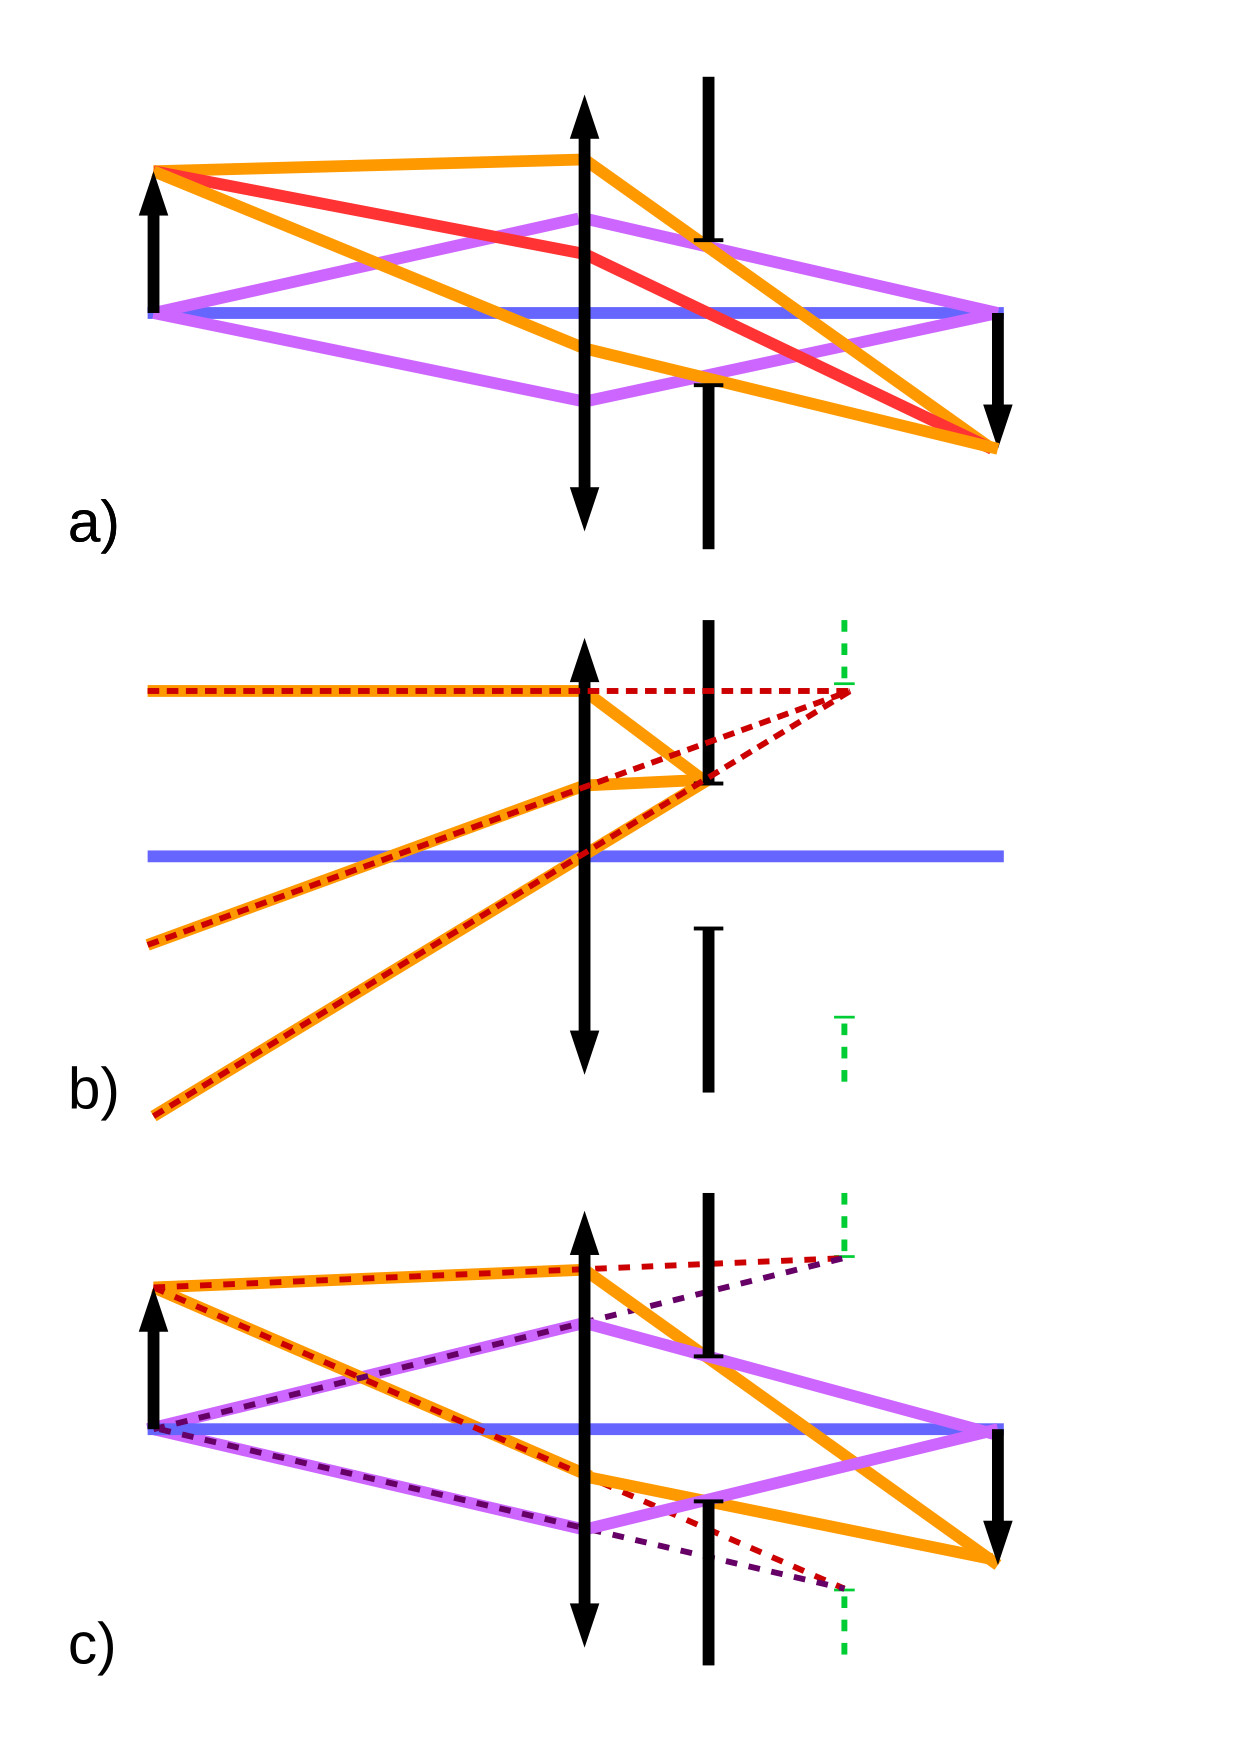
\includegraphics[width=0.5\columnwidth]{pupil}
  \caption{a) In an imaging system without vignetting, the stop acts as aperture for rays from all field points. The rays displayed are on-axis ray (blue), marginal rays (violet), chief ray (red), and coma rays (orange).
  b) In the system shown here, the lens creates a virtual image of the stop, the pupil (green).
  c) The imaging relation between pupil and stop causes rays aimed at the pupil border to be refracted onto the stop border.
  }
  \label{fig:pupil}
\end{figure}

The optical system is capable of transmitting only a certain angular spectrum of the light emitted by each object field point.
We call the component which limits the amount of transmitted light for the on-axis field point \emph{stop}.
The stop can be, for example, the clear aperture of a finite sized lens or a metal ring aperture.
If at field points far from the axis also other elements start to clip rays, we call this additional clipping \emph{vignetting}.

The rays emitted by the central (on-axis) field point that hit the border of the stop are called \emph{marginal rays}.
The rays emitted by any non-zero field point that hit the border of the stop are called \emph{coma rays}.
A ray emitted by any non-zero field point that hits the center of the stop is called \emph{chief ray}.
Often, the chief ray is approximated to be the central ray in the transmitted ray bundle emitted by a field point.

We call the plane containing the optical axis and the chief ray \emph{meridional} or \emph{tangential plane}, and the plane that contains the chief ray and is orthogonal to the meridional plane \emph{sagittal plane}.

We divide an optical system in two groups -- elements in front of and behind the stop. 
We consider both groups of optical elements as systems imaging the stop.
We call the image of the stop created by the object sided elements \emph{entrance pupil}, and the image created by the image sided elements \emph{exit pupil}.

Rays in the object and rays in the entrance pupil need to pass the same group of optical elements in order to reach the stop. 
We can regard the propagation of rays from the object to the stop as a free space propagation from the object to the entrance pupil and a subsequent imaging into the stop.
In close analogy, we can image rays from the stop to the exit pupil and perform a free-space propagation from the exit pupil to the image.
This property is often used to determine the marginal and coma angles: 
aiming from the object into the entrance pupil by free-space propagation is much easier than tracing rays from the object to the stop.
Care has to be taken if the front lens group imaging the stop to the pupil suffers from aberrations such as distortion.



\section{Direction of rays}
We assume rays propagate along the direction of energy transport, that is, the direction of the Poynting vector.
We assign a unit direction vector $\Vector{d}$ to each ray.
The direction vector points in the direction of the time averaged Poynting vector.
\begin{eqnarray}
 \Vector{d} &=& \frac{\timeavg{\Vector{S}}}{|\timeavg{\Vector{S}}|}
\end{eqnarray}
In general, the direction of the ray $\Vector{d}$ and its corresponding plane wave phase retardation $\Vector{k}$ may differ.

\section{Surface Normal}
Assume the surface of a material boundary is given in the form
\begin{eqnarray}
 z &=& z(x,y)
\end{eqnarray}
Two (infinitessimal) local in-plane vectors are 
\begin{eqnarray}
d\Vector{e}_1 = \begin{pmatrix}
                 dx \\ 0 \\ \frac{\partial z}{\partial x} dx
                \end{pmatrix}
\\
d\Vector{e}_2 = \begin{pmatrix}
                 0 \\ dy \\ \frac{\partial z}{\partial y} dy
                \end{pmatrix}
\end{eqnarray}
We normalize these local vectors and form the surface normal, perpendicular to both
\begin{eqnarray}
 \Vector{n} &=& \Vector{e}_1 \times \Vector{e}_2 \\
 &=& 
   \frac{1}{\sqrt{ 1 + \left( \frac{\partial z}{\partial x} \right)^2 + \left( \frac{\partial z}{\partial y} \right)^2 }}
   \begin{pmatrix}
    - \frac{\partial z}{\partial x} \\ - \frac{\partial z}{\partial y} \\ 1
   \end{pmatrix}
\end{eqnarray}

\section{Lagrange formalism}
\remark{todo: derive Fermat from Maxwell}
\remark{todo: derive Lagrange from Fermat}

Euler-Lagrange-Equations are given by
\begin{align}
 \frac{\text{d}}{\text{d}s} \frac{\partial \mathcal{L}}{\partial \Vector{r}'} &= \frac{\partial \mathcal{L}}{\partial \Vector{r}}\,.
\end{align}
The sloppy notation with vector derivatives means a differentiation by components.
\begin{align}
 \frac{\partial \mathcal{L}}{\partial \Vector{r}'} &= n(\Vector{r}(s)) \frac{\Vector{r}'(s)}{|\Vector{r}'(s)|} \stackrel{|\Vector{r}'(s)|=1}{=} n(\Vector{r}(s))\Vector{r}'(s)\,.
\end{align}
Therefore the appropriate differential equation (the so-called equation of motion, EOM) is given by
\begin{align}
 \frac{\text{d}}{\text{d}s} \left(n(\Vector{r}(s)) \frac{\text{d}\Vector{r}}{\text{d}s}\right) &= (\Vector{\nabla} n)(\Vector{r}(s)) \label{eq:ODEGRIN}\,.
\end{align}
( For a piecewise homogeneous medium the ODE system reduces to a system of algebraic equations 
[btw. this corresponds to a reduction of the
first variation of the integral to a first derivative of the corresponding sum].) 
For our later raytracing the initial conditions are given by:
\begin{subequations}
\label{eq:ODEGRINic}
\begin{align}
 \Vector{r}(s=0) &= (x,y,z)\,,\\
 \Vector{r}'(s=0) &= (d_x, d_y, \sqrt{1-d_x^2-d_y^2})\,,
\end{align}
\end{subequations}
where $\Vector{d}$ is the direction unit vector of some certain ray and $(x,y,z)$ is the starting position.
Now we may integrate \eqref{eq:ODEGRIN} for every set of initial conditions \eqref{eq:ODEGRINic}
and obtain after a (in general numerical) integration a set of values $\Vector{r}(s)$ and $\Vector{r}'(s)$
which correspond to the final position and direction of the ray.

\section{Hamilton formalism}
There are two distinct parametrisations. The first one parametrizes the theory with respect to the
arc length $s$ in 3D space where (one possible choice of) the Hamiltonian is given by
\begin{align}
 H &= \Vector{p}^2 - n^2 = 0\,.
\end{align}
The canonical momentum $\Vector{p}$ is given by $\Vector{p} = n \Vector{d}$. (From this consideration the constraint on
the Hamiltonian becomes clear, since $|\Vector{d}| = 1$.) The canonical equations are given by
\begin{subequations}
\label{eq:H3Deom}
\begin{align}
 \frac{\text{d}\Vector{q}}{\text{d}s} &= \frac{\partial H}{\partial \Vector{p}} = 2 \Vector{p}\,,\\
 \frac{\text{d}\Vector{p}}{\text{d}s} &= -\frac{\partial H}{\partial \Vector{q}} = 2 n (\Vector{\nabla} n)\,, 
\end{align}
\end{subequations}
The second parametrisation is given by the $z$ position with respect to the optical axis. Here the Hamiltonian is
given by
\begin{align}
 H_{\text{2D}} &= -n(\Vector{Q}, z)\sqrt{1 - \frac{\Vector{P}^2}{n(\Vector{Q}, z)^2}}\label{eq:Hamiltonian2D}\,,
\end{align}
and is equal to the negative component of the 3D momentum.
This comes from the Legendre transformation of the Lagrangian
\begin{align}
 \mathcal{L} &= n(\Vector{Q}, z) \sqrt{1 + V^2}\,,
\end{align}
now parametrized by $z$ as independent variable, $\Vector{Q} = (x,y)$ and $\Vector{V} = (x'(z), y'(z))$.
The Legendre transformation involves first an inversion of the relation
\begin{align}
 \Vector{P} &= \frac{\partial \mathcal{L}}{\partial \Vector{V}} = n(\Vector{Q}, z) \frac{\Vector{V}}{\sqrt{1 + \Vector{V}^2}}\,,
\end{align}
with respect to $\Vector{V}$ and afterwards the calculation of
\begin{align}
 H_{\text{2D}}(\Vector{Q}, \Vector{P},z) &= \scpm{\Vector{P}}{\Vector{V}(\Vector{P})} - \mathcal{L}(\Vector{Q}, z, \Vector{P})\,,
\end{align}
which leads to \eqref{eq:Hamiltonian2D}. The equations of motion due to the canonical formalism 
are therefore given by [remember $\Vector{Q} = (x,y)$, $\Vector{P} = n (d_x, d_y)$]
\begin{subequations}
\label{eq:H2Deom}
\begin{align}
 \frac{\text{d}\Vector{Q}}{\text{d}z} &= \frac{\partial H_{\text{2D}}}{\partial \Vector{P}} = \frac{\Vector{P}}{n \sqrt{1 - \frac{\Vector{P}^2}{n^2}}}\,,\\
 \frac{\text{d}\Vector{P}}{\text{d}z} &= -\frac{\partial H_{\text{2D}}}{\partial \Vector{Q}} = \frac{\Vector{\nabla}_{\Vector{Q}} n}{\sqrt{1 - \frac{\Vector{P}^2}{n^2}}}\,.    
\end{align}
\end{subequations}
In general $n = n(\Vector{Q}, z)$ holds, so the Hamiltonian depends explicitly on the independent variable.
Therefore for $z$ dependent $n$ the Hamiltonian is no conserved quantity anymore and
\begin{align}
 \frac{\partial H_{\text{2D}}}{\partial z} &= -\frac{\frac{\partial n}{\partial z}}{\sqrt{1 - \frac{\Vector{P}^2}{n^2}}}\,.
\end{align}
(For constant $n$ this formulation is very similar to the Hamiltonian formulation of a 
massive particle in special relativity with imaginary linear momentum.
Therefore nearly all of the results there are applicable here. It is also very useful 
for the paraxial approximation which corresponds to a post-Newtonian expansion.)

\section{Optical path length}
We define the optical path length as the time of travel of a near-monochromatic wavepacket times the vacuum speed of light.

In the special case of materials that can be described by an isotropic, real valued refractive index, the optical path length functional is given according to the Fermat principle,
\begin{align}
 L &= \int_{s_1}^{s_2} \underbrace{n(\Vector{r}(s)) |\Vector{r}'(s)|}_{=\mathcal{L}} \text{d}s\,.\label{eq:fermatiso}
\end{align}
with the corresponding ``Lagrangian'' $\mathcal{L}$.
$s$ is the arc length and therefore the derivative $\Vector{r}'(s)$ is a unit vector. (For the Euler Lagrange
equations we may not set it to $1$ at the moment.)

\remark{to do: all other cases; restriction to linear optics}

\section{Numerical Integration for GRIN Media}
Let us start with the integration of the 3D formulation since it is separable $H = T + U$. Here we use a symplectic integration formalism
due to its symmetry preserving phase space integration structure. For the details we kindly refer the reader to the
literature. A symplectic integrator for a separable Hamiltonian is given by the following scheme with time step $h$:
\begin{align}
 \begin{pmatrix}
  \Vector{q} \\
  \Vector{p}
 \end{pmatrix} \mapsto
 \begin{pmatrix}
  \Vector{q} + c_i h \frac{\partial T}{\partial \Vector{p}} \\
  \Vector{p}
 \end{pmatrix}
\end{align}
and succesively
\begin{align}
 \begin{pmatrix}
  \Vector{q} \\
  \Vector{p}
 \end{pmatrix} \mapsto
 \begin{pmatrix}
  \Vector{q} \\
  \Vector{p} - d_i h \frac{\partial U}{\partial \Vector{q}}
 \end{pmatrix}\,.
\end{align}
For a fourth order scheme $i=1\dots4$ and the coefficients are given by
\begin{align}
 c_1 = c_4 = \frac{1}{2(2 - 2^{1/3})}\,,\\
 c_2 = c_3 = \frac{1 - 2^{1/3}}{2(2 - 2^{1/3})}\,,\\
 d_1 = d_3 = \frac{1}{2 - 2^{1/3}}\,,\\
 d_2 = -\frac{2^{1/3}}{2 - 2^{1/3}}\,\quad d_4 = 0\,.
\end{align}
For a further improvement it may be necessary to use adaptive ``time'' steps.
These can be implemented, e.g., by an extension of the phase space where
the time is an additional canonical coordinate. The extension is achieved by
a so-called Sundman transformation (which is in fact a Poincar{\'e} transformation)
of the ``time'' coordinate
$\text{d}s/\text{d}\sigma = g(\Vector{q}, \Vector{p})$.
By using a special form of this transformation $g$ the new Hamiltonian is separable and we
may use a symplectic scheme like the one mentioned above to integrate the new formulation.

\section{Paraxial Optics}
In paraxial optics, we consider centro-symmetric systems with rays close to the optical axis both in real and angular space. 
Parabasal optics decribes rays close to a base ray. 
We describe small fields around the base ray,
allowing for systems with decenter, tilts and freeshapes. 

\subsection{ABCD formalism}
We consider a centro-symmetric optical system. 
That is, all optical elements are symmetric around a common optical axis.
All meridional planes are equivalent.
Without loss of generality, we choose our $z$-axis along the optical axis and consider the meridional $yz$ plane only.
We describe our rays by a $y$ coordinate and its inclination $y^{\,\prime} = \partial y / \partial z$. 
We only consider rays with zero out of plane ($x$) coordinates and directions.
Disregarding sagittal rays, we cannot describe astigmatism in the ABCD formalism.

The ray on the optical axis, $y=0, y^{\,\prime}=0$, is not refracted in the centro-symmetric system.
The next leading order for rays with small height and angle is the linear order, so our model of an optical element in paraxial approximation is

\begin{eqnarray}
 \begin{pmatrix}
  y \\ y^{\,\prime}
 \end{pmatrix}
 &=&
 \begin{pmatrix}
  A & B \\ C & D
 \end{pmatrix}
 \begin{pmatrix}
  y_0 \\ y_0^{\,\prime}
 \end{pmatrix}
\end{eqnarray}

Performing the Taylor expansion in linear order, we find the ABCD-Matrices of typical optical elements. 
\begin{eqnarray}
 \begin{pmatrix}
  1 & \Delta z \\ 0 & 1
 \end{pmatrix}
 && \textrm{propagation in homogeneous media}
 \\
 \begin{pmatrix}
  1 & 0 \\ \left( \frac{n_1}{n_2} - 1 \right) \frac{1}{R} & \frac{n_1}{n_2}
 \end{pmatrix}
 && \textrm{refraction of a thin surface}
 \\
 \begin{pmatrix}
  1 & 0 \\ -\frac{2}{R} & 1
 \end{pmatrix}
 && \textrm{thin mirror}
 \\
 \begin{pmatrix}
  1 & 0 \\ -\frac{1}{f} & 1
 \end{pmatrix}
 && \textrm{thin lens without immersion}
\end{eqnarray}
Propagation in homogeneous media does not change the ray direction, and refraction at thin surfaces (surfaces with negligible sag) does not change the ray position.

An optical system can be described as concatenation of its optical elements.

\begin{eqnarray}
 \begin{pmatrix}
  y_{im} \\ y_{im}^{\,\prime}
 \end{pmatrix}
 &=&
 \begin{pmatrix}
  A_N & B_N \\ C_N & D_N
 \end{pmatrix}
 \cdot
 ...
 \cdot
 \begin{pmatrix}
  A_2 & B_2 \\ C_2 & D_2
 \end{pmatrix}
 \cdot
 \begin{pmatrix}
  A_1 & B_1 \\ C_1 & D_1
 \end{pmatrix}
 \cdot
 \begin{pmatrix}
  y_{obj} \\ y_{obj}^{\,\prime}
 \end{pmatrix}
\end{eqnarray}
Where the index $1$ describes the element closest to the object.
The elements can be air gaps, single surfaces, or complete lens assemblies.

\subsection{Interpretation of ABCD matrices}
Let's consider we have a given ABCD matrix of an optical system and want to know the system's first order optical properties.

\begin{eqnarray}
  y_{im} &=& A y_{obj} + B y_{obj}^{\,\prime}
  \\ 
  y_{im}^{\,\prime} &=& C y_{obj} + D y_{obj}^{\,\prime}
\end{eqnarray}

\subsubsection{Focal Length}
We consider a collimated ray bundle $y_{obj}^{\,\prime} = 0$.
We define the image sided paraxial focal length as the distance between image sided principal plane and image.
In the principal plane, the collimated marginal ray has the height $y_{obj}$ and inclination $y_{im}^{\,\prime}$, bending towards the focal point.
\begin{eqnarray}
 f_{im} &:=& - \frac{ y_{obj} }{ y_{im}^{\,\prime} } 
 \\
 f_{im} &=& - \frac{ 1 }{ C } \\ 
\end{eqnarray}

To determine the object sided focal length, we illuminate the system with a collimated beam from the image side $y_{im}^{\,\prime}=0$.
\begin{eqnarray}
 \begin{pmatrix}
  A & B \\ C & D
 \end{pmatrix}^{-1}
 \cdot
 \begin{pmatrix}
  y_{im} \\ y_{im}^{\,\prime}
 \end{pmatrix}
 &=&
 \begin{pmatrix}
  y_{obj} \\ y_{obj}^{\,\prime}
 \end{pmatrix}
\\
  \begin{pmatrix}
  A & B \\ C & D
 \end{pmatrix}^{-1}
 &=&
 \frac{1}{AD-BC}
  \begin{pmatrix}
  D & - B \\ -C & A
 \end{pmatrix}
\end{eqnarray}
We obtain in close analogy to the image sided focal length
\begin{eqnarray}
 f_{obj} &=& - \frac{AD-BC}{C}
\end{eqnarray}
In systems with classical lens elements only and without immersion, 
we find equal focal lengths on object and image side. The determinant of the ABCD matrix is then equal to one.

\subsubsection{Finite Conjguate Systems}
In object sided finite conjugate systems, each point in object space $y_{obj}$ is a field point, 
emitting a cone of rays $y_{obj}^{\,\prime}$.

Imaging is achieved, if rays cast from an object sided field point are joined in an image sided point.
The image point is reached independently from the ray direction in the object plane.

\begin{eqnarray}
   y_{im} &=& A y_{obj} \\
   B &=& 0
\end{eqnarray}

We call $A = y_{im} / y_{obj}$ magnification of the system.
$A$ is unitless.
Once the imaging condition is fulfilled, all rays originating from an object field point are focused stigmatically to the corresponding image point. 
The ABCD formalism calculates first order properties only.
If the ABCD matrices are calculated with a corresponding dispersion model, lateral and transversal first order chromatic aberrations can be modeled.
Also, the paraxial ABCD ray trace may be the basis for calculating the Seidel coefficients.

In case $B$ is nonzero, the imaging condition can often be achieved by changing an air gap size. Most often the image sided distance is refocused.
\begin{eqnarray}
 \begin{pmatrix}
  \tilde{A} & \tilde{B} \\ \tilde{C} & \tilde{D}
 \end{pmatrix}
 =
 \begin{pmatrix}
  1 & \Delta z_{im} \\ 0 & 1
 \end{pmatrix}
 \cdot
 \begin{pmatrix}
  A & B \\ C & D
 \end{pmatrix}
 &=&
  \begin{pmatrix}
  A + C \Delta z_{im} & B + D \Delta z_{im} \\ C & D
 \end{pmatrix}
 \label{eq:abcd_refocusing}
\end{eqnarray}
We choose $\Delta z_{im} = - B / D $. Note that $\tilde{A}$ is equal to the magnification \emph{only} if the imaging condition is met. 
Otherwise, the matrix element has no physical meaning.
In particular, it is unsuitable to deduct information about the telecentricity of an imaging system.
The magnifictaion $\tilde{A}$ after refocusing is
\begin{eqnarray}
 \tilde{A} &=& A - \frac{BC}{D}
\end{eqnarray}



\subsubsection{Infinite to Finite Conjguate Systems}
In object sided infinite conjugate systems, each direction in object space $y^{\,\prime}_{obj}$ corresponds to a field point, 
emitting a collimated bundle of rays.

\begin{eqnarray}
   y_{im} &=& B y^{\,\prime}_{obj} \\
   A &=& 0
\end{eqnarray}

We call $B = y_{im} / y^{\,\prime}_{obj}$ magnification of the system.
The unit of $B$ is length units per radian.

In case the imaging condition $A=0$ is not achieved, we try to refocus the last surface (see eq. \ref{eq:abcd_refocusing}).
We choose $\Delta z_{im} = - A / C $.
The magnifictaion $\tilde{B}$ after refocusing is
\begin{eqnarray}
 \tilde{B} &=& B - \frac{AD}{C} 
\end{eqnarray}
In systems with classical lens elements only and no immersion, the determinant of the ABCD matrix is 1, and the magnification simplifies to
\begin{eqnarray}
 \tilde{B} &=& - \frac{1}{C} 
\end{eqnarray}


\subsubsection{Finite to Infinite Conjguate Systems}
In image sided infinite conjugate systems, each point in object space $y_{obj}$ emits a cone of rays, 
that is collimated by the optical system.

\begin{eqnarray}
   y^{\,\prime}_{im} &=& C y_{obj} \\
   D &=& 0
\end{eqnarray}

We call $C = y^{\,\prime}_{im} / y_{obj}$ magnification of the system.
The unit of $C$ is radian per length unit.
In case $D$ is nonzero, we try to fulfill the imaging condition by adding an object sided air gap.
\begin{eqnarray}
 \begin{pmatrix}
  \tilde{A} & \tilde{B} \\ \tilde{C} & \tilde{D}
 \end{pmatrix}
 =
 \begin{pmatrix}
  A & B \\ C & D
 \end{pmatrix}
 \cdot
  \begin{pmatrix}
  1 & \Delta z_{obj} \\ 0 & 1
 \end{pmatrix}
 &=&
 \begin{pmatrix}
  A\qquad & A \Delta z_{obj} + B \\
  C\qquad & C \Delta z_{obj} + D 
 \end{pmatrix}
\end{eqnarray}
We choose $\Delta z_{obj} = - D / C$.
The magnifictaion $\tilde{C}$ after shifting the object distance is
\begin{eqnarray}
 \tilde{C} &=& C 
\end{eqnarray}


\subsubsection{Infinite Conjguate Systems}
In both sided infinite conjugate systems, imaging is achieved if collimated ray bundles are transfered into collimated ray bundles.

\begin{eqnarray}
   y^{\,\prime}_{im} &=& D y^{\,\prime}_{obj} \\
   C &=& 0
\end{eqnarray}

We call $D = y_{im} / y^{\,\prime}_{obj}$ angular magnification of the system.
$D$ is unitless.

An infinite to infinite system cannot be refocused by adding a finite air distance on either object or image side.

\section{Parabasal Optics}

\subsection{Pilot Ray Concept}

\subsubsection{Motivation}

The ABCD ansatz allows for very fast calculations and is invaluable in the pre-design stage.
Its simplicity, however, comes with the restriction to meridional rays in centro-symmetric systems and the need for an optical axis.

In systems like Offner systems or off-axis parabolic mirrors, the center-of-field chief ray is no more aligned with the axis of rotational symmetry of the surfaces.
In these systems, it is no longer sufficient to obtain first order properties from the central curvature on the axis of symmetry of each surface.
In other systems, like freeshape Schiefspiegler telescopes, there is no axis of symmetry at all. 
Anamorphotic systems, on the other hand, often have an optical axis, but do not have the same effective surface curvature in all meridional planes.

In this section, we develop a description for the first order properties of optical systems 
and describe rotationally symmetric and non-symmetric systems with a single formalism.
It is a formalism for rays close to the center-of-field chief ray, which we call \emph{pilot ray} in the following.
This pilot ray takes the role of the optical axis in rotationally symmetric systems. 
By choosing the term pilot ray, we want to avoid confusions with mechanical symmetry axes of sub-systems.
In many systems, the intial pilot ray direction is perpendicular to the object plane. 
An exception is found, for example, in Scheimpflug systems.



\subsubsection{Propagation of rays through an optical system}
Our ansatz is to perform a real ray trace of the pilot ray and describe a small area around it by a Taylor expansion around the real ray intersection point.
From this Taylor expansion, we derive first order properties, like focal length, magnification, aperture size, pupils, and image position.
The concept is a parabasal approximation around a non-paraxial pilot ray.
It is a generalization of the ABCD formalism. 
We describe the vectorial deviation from the pilot ray position and direction.
We consider near-pilot rays, that have an intersection point and a wavevector close to the pilot ray.

\begin{tabular}{ l | l | l }
		    & pilot ray & near-pilot ray \\
& & \\ \hline & & \\
intersection point  & $\Vector{r}_{pilot}$ & ${\Vector{r}} = \Vector{r}_{pilot} + \Delta\Vector{r}$ \\
wavevector  & $\Wavevector_{pilot}$ & ${\Wavevector} = \Wavevector_{pilot} + \Delta\Wavevector$ \\
ray direction  & $\Vector{d}_{pilot}$ & ${\Vector{d}} = \Vector{d}_{pilot} + \Delta\Vector{d}$ \\
surface normal      & $\Vector{n}_{pilot} = \Vector{n}(\Vector{r}_{pilot})$ & ${\Vector{n}} = \Vector{n}({\Vector{r}}) = \Vector{n}_{pilot} + \Delta\Vector{n}$ \\
\end{tabular}\\[2ex]
We represent the propagation of these deviations through the optical system by a propagation operator $\hat{G}$
\begin{eqnarray}
 \begin{pmatrix}
  \Delta \Vector{r}_{im} \\ \Delta \Wavevector_{im}
 \end{pmatrix}
 &=&
 \hat{G}
 \begin{pmatrix}
  \Delta \Vector{r}_{obj} \\ \Delta \Wavevector_{obj}
 \end{pmatrix}
\end{eqnarray}
By definition, the propagator $\hat{G}$ projects the object sided pilot ray onto the image sided pilot ray.
That is $\hat{G}\Vector{0} = \Vector{0}$.
In analogy to the ABCD formalism, we neglect terms quadratic in the change of direction or position, 
$\orderof{\Delta\Wavevector^2}$ and $\orderof{\Delta\Vector{r}^2}$, as well as mixed terms $\orderof{\Delta\Wavevector\Delta\Vector{r}}$.
The linear terms in $\hat{G}$ can be represented by a matrix,
and we can express the effect of multiple propagators as the product of its matrices.
The individual propagators can be, for example, free space propagation or surface refraction.

\begin{eqnarray}
 \begin{pmatrix}
  \Delta \Vector{r}_{im} \\ \Delta \Wavevector_{im}
 \end{pmatrix}
 &=&
 \hat{G}_N \cdot \hat{G}_{N-1} \cdot ... \cdot \hat{G}_3 \cdot \hat{G}_2 \cdot \hat{G}_1 \cdot
 \begin{pmatrix}
  \Delta \Vector{r}_{obj} \\ \Delta \Wavevector_{obj}
 \end{pmatrix}
\end{eqnarray}

In general, the matrices do not commutate. $\hat{G}_1$ is the propagator closest to the object.
In the following, we discuss the rank of the matrices $\hat{G}$ and the basis of $\Delta \Vector{r}$ and $\Delta \Wavevector$.


\subsubsection{Near-Pilot Basis Systems}

The deviations may not be chosen freely, but we need to choose
$\Delta\Vector{r}$, $\Delta\Wavevector$ and $\Delta\Vector{d}$ 
in a way so that both pilot and near-pilot rays
have valid properties.
Intersection points must lay on the surface,
wavevectors must obey the dispersion relation 
and ray direction vectors must be of unit length.
This limits the degrees of freedom for the deviations.

\paragraph{Intersection points}

We demand that near-pilot intersection points are on the surface.
In parabasal approximation, we assume each surface planar in a small area around the pilot ray intersection point. 
We represent the ray height in this plane by
\begin{eqnarray}
 \Delta\Vector{r} = X \Vector{e}_{X} + Y \Vector{e}_{Y}
 \label{eq:deltaR_equals_XY}
\end{eqnarray}
where $\Vector{e}_{X}$ and $\Vector{e}_{Y}$ are in the tangential surface plane.

\paragraph{Wavevectors}
Both pilot and near-pilot wavevector must fulfill the dispersion relation. 
In contrast to the real valued ray directions, wavevectors may be complex valued.

\paragraph{Isotropic, homogenous media.}

The dispersion in isotropic media reads
\begin{eqnarray}
 \Wavevector \cdot \Wavevector &=& \Wavevector_{pilot} \cdot \Wavevector_{pilot} = \omega^2 \vacuumpermeability \scalarpermittivity
\end{eqnarray}
Near-pilot rays must fulfill
\begin{eqnarray}
 \Delta \Wavevector \cdot \Wavevector_{pilot} &=& 0 + 0i
\end{eqnarray}

\paragraph{Anisotropic, homogeneous media.}
TODO

\paragraph{Wavevector Degrees of Freedom}
The change of the wavevector $\Delta\Wavevector$ is a 3 dimensional vector of complex numbers, that is, 6 real valued degrees of freedom.
The dispersion, as discussed in the paragraphs above, is a scalar complex valued equation, imposing 2 real valued constraints.

We represent the remaining degrees of freedom of $\Delta \Wavevector$ as
\begin{eqnarray}
 \Delta \Wavevector &=& U \Vector{e}_U + V \Vector{e}_V
\end{eqnarray}
where $\Vector{e}_U$ and $\Vector{e}_V$ are independent basis vectors and $U,V$ are complex valued prefactors.
\remark{TODO:Check whether this representation is possible also for the general anisotropic case.}
The basis vectors $\Vector{e}_U, \Vector{e}_V$ are defined up to a complex valued global phase and a roll degree of freedom. 


\subsubsection{XYUV matrices}
We choose the object sided basis vectors $\Vector{e}_{X,obj}, \Vector{e}_{Y,obj}, \Vector{e}_{U,obj}, \Vector{e}_{V,obj}$ 
in a way that both pilot and near-pilot rays start in the object plane and obey the dispersion relation, 
as described in the previous section.
We trace the pilot ray to the final surface 
and define the near-pilot basis vectors in the final plane $\Vector{e}_{X,fin}, \Vector{e}_{Y,fin}, \Vector{e}_{U,fin}, \Vector{e}_{V,fin}$.
The propagator for near-pilot rays is the Jacobi matrix
\begin{eqnarray}
 \begin{pmatrix}
  X_{fin} \\[2ex] Y_{fin} \\[2ex] \Re U_{fin}\\[2ex] \Re V_{fin} \\[2ex] \Im U_{fin} \\[2ex] \Im V_{fin} 
 \end{pmatrix}
 &=&
 \begin{pmatrix}
  \frac{\partial X_{fin}}{\partial X_{obj}} & \frac{\partial X_{fin}}{\partial Y_{obj}} & \frac{\partial X_{fin}}{\partial \Re U_{obj}} & \frac{\partial X_{fin}}{\partial \Re V_{obj}} & \frac{\partial X_{fin}}{\partial \Im U_{obj}} & \frac{\partial X_{fin}}{\partial \Im V_{obj}} \\[2ex]
  \frac{\partial Y_{fin}}{\partial X_{obj}} & \frac{\partial Y_{fin}}{\partial Y_{obj}} & \frac{\partial Y_{fin}}{\partial \Re U_{obj}} & \frac{\partial Y_{fin}}{\partial \Re V_{obj}} & \frac{\partial Y_{fin}}{\partial \Im U_{obj}} & \frac{\partial Y_{fin}}{\partial \Im V_{obj}} \\[2ex]
  \frac{\partial \Re U_{fin}}{\partial X_{obj}} & \frac{\partial \Re U_{fin}}{\partial Y_{obj}} & \frac{\partial \Re U_{fin}}{\partial \Re U_{obj}} & \frac{\partial \Re U_{fin}}{\partial \Re V_{obj}} & \frac{\partial \Re U_{fin}}{\partial \Im U_{obj}} & \frac{\partial \Re U_{fin}}{\partial \Im V_{obj}} \\[2ex]
  \frac{\partial \Re V_{fin}}{\partial X_{obj}} & \frac{\partial \Re V_{fin}}{\partial Y_{obj}} & \frac{\partial \Re V_{fin}}{\partial \Re U_{obj}} & \frac{\partial \Re V_{fin}}{\partial \Re V_{obj}} & \frac{\partial \Re V_{fin}}{\partial \Im U_{obj}} & \frac{\partial \Re V_{fin}}{\partial \Im V_{obj}} \\[2ex]
  \frac{\partial \Im U_{fin}}{\partial X_{obj}} & \frac{\partial \Im U_{fin}}{\partial Y_{obj}} & \frac{\partial \Im U_{fin}}{\partial \Re U_{obj}} & \frac{\partial \Im U_{fin}}{\partial \Re V_{obj}} & \frac{\partial \Im U_{fin}}{\partial \Im U_{obj}} & \frac{\partial \Im U_{fin}}{\partial \Im V_{obj}} \\[2ex]
  \frac{\partial \Im V_{fin}}{\partial X_{obj}} & \frac{\partial \Im V_{fin}}{\partial Y_{obj}} & \frac{\partial \Im V_{fin}}{\partial \Re U_{obj}} & \frac{\partial \Im V_{fin}}{\partial \Re V_{obj}} & \frac{\partial \Im V_{fin}}{\partial \Im U_{obj}} & \frac{\partial \Im V_{fin}}{\partial \Im V_{obj}}
 \end{pmatrix}
 \begin{pmatrix}
  X_{obj} \\[2ex] Y_{obj} \\[2ex] \Re U_{obj} \\[2ex] \Re V_{obj} \\[2ex] \Im U_{obj} \\[2ex] \Im V_{obj} 
 \end{pmatrix} \nonumber \\
\end{eqnarray}
We obtain this matrix by multiplying the matrices of all atomic propagation, refraction, reflection, and coordinate transformation operations.
To obtain these atomic matrices, we perform Taylor expansions around the pilot ray.
For systems where an explicit calculation is not possible
-- or the operator suffers from laziness --
it can be approximated by differential quotients of real ray traces of rays with small but finite differences.

We abbreviate the coefficients of the propagator by sub-matrices $\hat{A}, \hat{B}, \hat{C}, \hat{D}$, 
resembling the ABCD formalism.
\begin{eqnarray}
 \begin{pmatrix}
  X_{fin} \\ Y_{fin} \\ \Re U_{fin} \\ \Re V_{fin} \\ \Im U_{fin} \\ \Im V_{fin} 
 \end{pmatrix}
 &=&
 \begin{pmatrix}
  A_{11} & A_{12} & B_{11} & B_{12} & B_{13} & B_{14} \\
  A_{21} & A_{22} & B_{21} & B_{22} & B_{23} & B_{24} \\
  C_{11} & C_{12} & D_{11} & D_{12} & D_{13} & D_{14} \\
  C_{21} & C_{22} & D_{21} & D_{22} & D_{23} & D_{24} \\
  C_{31} & C_{32} & D_{31} & D_{32} & D_{33} & D_{34} \\
  C_{41} & C_{42} & D_{41} & D_{42} & D_{43} & D_{44}
 \end{pmatrix}
 \begin{pmatrix}
  X_{obj} \\ Y_{obj} \\ \Re U_{obj} \\ \Re V_{obj} \\ \Im U_{obj} \\ \Im V_{obj} 
 \end{pmatrix}
\end{eqnarray}


\subsubsection{Propagation in homogeneous media}
In homogeneous media, rays travel along straights.
That is, wavevector and ray direction do not change.
We consider the propagation between 2 parallel planes, 
separated by a pilot ray geometric path length of $\Delta s$
\begin{eqnarray}
 \hat{G}_{prop} &=&
 \begin{pmatrix}
  1 & 0 & \frac{\partial^2 X}{\partial s \partial \Re U} \Delta s & \frac{\partial^2 X}{\partial s \partial \Re V} \Delta s & \frac{\partial^2 X}{\partial s \partial \Im U} \Delta s & \frac{\partial^2 X}{\partial s \partial \Im V} \Delta s \\[2ex]
  0 & 1 & \frac{\partial^2 Y}{\partial s \partial \Re U} \Delta s & \frac{\partial^2 Y}{\partial s \partial \Re V} \Delta s & \frac{\partial^2 Y}{\partial s \partial \Im U} \Delta s & \frac{\partial^2 Y}{\partial s \partial \Im V} \Delta s \\[2ex]
  0 & 0 & 1 & 0 & 0 & 0 \\[2ex]
  0 & 0 & 0 & 1 & 0 & 0 \\[2ex]
  0 & 0 & 0 & 0 & 1 & 0 \\[2ex]
  0 & 0 & 0 & 0 & 0 & 1 \\[2ex]  
 \end{pmatrix}
 \label{eq:xyuv_propagation_homogeneous}
\end{eqnarray}

\subsection{Interpretation of XYUV matrices}
\subsubsection{Focal Length}
TODO

\subsubsection{Finite Conjugate Systems}
We define imaging as:
For a fixed ray starting position $(X,Y)$, there is a fan $(U,V)$ that is propagated on a common point in image space.

\begin{eqnarray}
 \begin{pmatrix}
  X_{im} \\ Y_{im} 
 \end{pmatrix}
 &=&
 \hat{A}
 \begin{pmatrix}
  X_{obj} \\ Y_{obj}
 \end{pmatrix}
\end{eqnarray}
or, in other words,
\begin{eqnarray}
 \hat{B}
 \begin{pmatrix}
  U_{obj} \\ V_{obj}
 \end{pmatrix}
 &=& 
 0
\end{eqnarray}
The matrix $\hat{B}$ is of rank 2, the input vector $(U,V)$ contains 4 independent real valued degrees of freedom.
That is, we can impose more constraints on the input vector. 
In the following, we develop these additional requirements.

We consider the plane waves of the pilot ray and a near pilot ray, 
$\Wavevector_{pilot}$ and $\Wavevector = \Wavevector_{pilot} + U \Vector{e}_U + V \Vector{e}_V$.
They interfere and form a sinusoidal grating intensity pattern
\begin{eqnarray}
 I &=& |\Efield_{0,pilot}|^2 + |\Efield_{0}|^2 + 2 \Re \left( \overline{\Efield}_{0}\Efield_{0,pilot} \exp(i(\Wavevector_{pilot} - \Wavevector)\Location) \right)
\end{eqnarray}
We restrict the locations to the image plane
\begin{eqnarray}
 \Location &=& \Location_{pilot} + X \Vector{e}_X + Y \Vector{e}_Y
\end{eqnarray}
We desire the modulation depth of the intensity pattern to be independent of position
\begin{eqnarray}
 (\Wavevector_{pilot} - \Wavevector)(X \Vector{e}_X + Y \Vector{e}_Y) \in \mathbb{R}
\end{eqnarray}
%\begin{eqnarray}
% \Im (U \Vector{e}_U + V \Vector{e}_V)(X \Vector{e}_X + Y \Vector{e}_Y) &=& 0
%\end{eqnarray}
Together with the imaging condition, we obtain
\begin{eqnarray}
  \begin{pmatrix}
  B_{11} & B_{12} & B_{13} & B_{14} \\
  B_{21} & B_{22} & B_{23} & B_{24} \\
  (\Im \Vector{e}_U) \Vector{e}_X & (\Im \Vector{e}_V) \Vector{e}_X & (\Re \Vector{e}_U) \Vector{e}_X & (\Re \Vector{e}_V) \Vector{e}_X \\
  (\Im \Vector{e}_U) \Vector{e}_Y & (\Im \Vector{e}_V) \Vector{e}_Y & (\Re \Vector{e}_U) \Vector{e}_Y & (\Re \Vector{e}_V) \Vector{e}_Y
 \end{pmatrix}
 \begin{pmatrix}
  \Re U_{obj} \\ \Re V_{obj} \\ \Im U_{obj} \\ \Im V_{obj} 
 \end{pmatrix}
 &=& 0
\end{eqnarray}
Nontrivial solutions are found if the determinant vanishes.
In case the determeninant is nonzero, 
we refocus by inserting a homogeneous material propagation (eq. \ref{eq:xyuv_propagation_homogeneous}) in front of the image plane.
\begin{eqnarray}
  \begin{vmatrix}
  B_{11} + \frac{\partial^2 X}{\partial s \partial \Re U} \Delta s & 
  B_{12} + \frac{\partial^2 X}{\partial s \partial \Re V} \Delta s & 
  B_{13} + \frac{\partial^2 X}{\partial s \partial \Im U} \Delta s & 
  B_{14} + \frac{\partial^2 X}{\partial s \partial \Im V} \Delta s \\[2ex]
  B_{21} + \frac{\partial^2 Y}{\partial s \partial \Re U} \Delta s & 
  B_{22} + \frac{\partial^2 Y}{\partial s \partial \Re V} \Delta s & 
  B_{23} + \frac{\partial^2 Y}{\partial s \partial \Im U} \Delta s & 
  B_{24} + \frac{\partial^2 Y}{\partial s \partial \Im V} \Delta s \\[2ex]
  (\Im \Vector{e}_U) \Vector{e}_X & (\Im \Vector{e}_V) \Vector{e}_X & (\Re \Vector{e}_U) \Vector{e}_X & (\Re \Vector{e}_V) \Vector{e}_X \\[2ex]
  (\Im \Vector{e}_U) \Vector{e}_Y & (\Im \Vector{e}_V) \Vector{e}_Y & (\Re \Vector{e}_U) \Vector{e}_Y & (\Re \Vector{e}_V) \Vector{e}_Y
 \end{vmatrix}
 &=& 0 \nonumber \\
\end{eqnarray}
The characteristic polynomial is quadratic in $\Delta s$, so we expect two defocus positions where the determinant vanishes.
The corresponding eigenvector $(U,V)$ forms a ray fan that is imaged to a point in the image plane.
Wavevectors with deviations orthogonal to the eigenvector, however, are in general not stigmatically imaged.
We obtain an anastigmatic line focus.
In case of degenerate solutions $\Delta s$, changes along both eigenvector directions are stigmatically focused. 


\chapter{Raytracing}

Classical raytracing through stepwise homogeneous media consists of the following steps: 
The ray is considered a straight in 3D space. 
First its intersection point with the next surface is calculated geometrically. 
Then, a new wavevector is determined using the refraction law for plane waves on planar surfaces.


\section{Intersections of Straights with Spheres, Aspheres and Free-shapes}\label{subsec:intersectionformulas}

\subsection{Biconics}
The word ``conic" is short for conic section. 
This refers to intersections of a plane with a cone.
A biconic describes a surface with two perpendicular sections of conic shape. 
These surfaces have two symmetry planes.
The explicit surface sag formula is given by
\begin{align}
 z &= \frac{\rho_x x^2 + \rho_y y^2}{1 + \sqrt{1 - (1+c_x) \rho_x^2 x^2 - (1+c_y) \rho_y^2 y^2}} \label{eq:biconic}\,.
\end{align}
The variables are $\rho_x = 1/R_x$ the $x$ curvature, $\rho_y = 1/R_y$ the $y$ curvature, $c_x$ the conic constant in $x$ direction,
and $c_y$ the conic constant in $y$ direction, respectively. 

Depending on the conic constant, the biconic $x$ and $y$ cross sections are a
\begin{eqnarray*}
     c < -1 && \textrm{hyperbola} \\
     c = -1 && \textrm{parabola} \\
-1 < c < 0 && \textrm{prolate ellipse} \\
     c = 0 && \textrm{sphere} \\
 0 < c < 1 && \textrm{oblate ellipse}
\end{eqnarray*}


An invariant or implicit form of the biconic sag equation \eqref{eq:biconic} is given by
\begin{align}
 (a(x,y) - 1) z^2 + (z - b(x,y))^2 &= 0\,,\label{eq:biconicImplicitSag}
\end{align}
where $a(x,y) = (1 + c_x) \rho_x^2 x^2 + (1 + c_y) \rho_y^2 y^2$ and $b(x,y) = \rho_x x^2 + \rho_y y^2$. 
Next we consider the ray straight equation
\begin{eqnarray}
 \Location &=& \Location_0 + \Vector{d} t \label{eq:ray}
\end{eqnarray}
$\Location_0$ is the ray start point, $\Vector{d}$ the ray direction unit vector and $t$ the free parameter of the straight.

Inserting the straight equation leads to a polynomial of fourth order in $t$.
The fourth order equation can be solved either analytically or numerically.
The one physically valid solution must be real valued.

\remark{to do: surface normal equation for all surface shapes}

\subsection{Simplified Biconic}
We assume a Biconic sag equation \eqref{eq:biconic} in which not all parameters are independent, but the x and y conic constants are linked via
\begin{eqnarray}
 \kappa := (1 + c_x) \rho_x = (1 + c_y) \rho_y
\end{eqnarray}
The coeffcients $a$ and $b$ in the implicit form of the sag equation \ref{eq:biconicImplicitSag} are no longer independent.
\begin{eqnarray}
 a(x,y) &=& \kappa b(x,y) 
\end{eqnarray}

We factor out the invariant sag equation \ref{eq:biconicImplicitSag}

\begin{eqnarray}
 %(a(x,y) - 1) z^2 + (z - b(x,y))^2 &=& 0 \\
 %(a - 1) z^2 + (z - b)^2 &=& 0 \\ 
 %a z^2 - z^2 + z^2 - 2 z b + b^2 &=& 0 \\ 
 (\kappa b) z^2 - 2 z b + b^2 &=& 0 
\end{eqnarray}
and divide this equation by $b$. Care has to be taken for the special case $b=0$. The division reduces the equation from a fourth to second order equation in $(x,y,z)$.
\begin{eqnarray}
 \kappa z^2 - 2 z + b &=& 0
\end{eqnarray}
Inserting the straight equation yields
\begin{eqnarray}
 %(1 + c_x) \rho_x z^2 - 2 z + \rho_x x^2 + \rho_y y^2 &=& 0 \\
 %\kappa z^2 - 2 z + \rho_x x^2 + \rho_y y^2 &=& 0 \\
 %\kappa (z_0+d_z t)^2 - 2 (z_0+d_z t) + \rho_x (x_0+d_x t)^2 + \rho_y (y_0+d_y t)^2 &=& 0 \\
 %\kappa ( z_0^2 + 2 z_0 d_z t + d_z^2 t^2 ) - 2 z_0 - 2 d_z t + \rho_x (x_0^2 +2 x_0 d_x t + d_x^2 t^2) + \rho_y (y_0^2 + 2 y_0 d_y t + d_y^2 t^2) &=& 0 \\
 %\kappa z_0^2 + 2 \kappa z_0 d_z t + \kappa d_z^2 t^2 - 2 z_0 - 2 d_z t + \rho_x x_0^2 + 2 \rho_x x_0 d_x t + \rho_x d_x^2 t^2 + \rho_y y_0^2 + 2 \rho_y y_0 d_y t + \rho_y d_y^2 t^2 &=& 0 \\
 %\left(   \kappa d_z^2 + \rho_x d_x^2 + \rho_y d_y^2   \right) t^2
 %  + 2 \left(  \kappa z_0 d_z - d_z  + \rho_x x_0 d_x + \rho_y y_0 d_y \right) t
 %  + \left( \kappa z_0^2 - 2 z_0 + \rho_x x_0^2 + \rho_y y_0^2 \right) 
 %  &=& 0 \\
 %\left(   \rho_x d_x^2 + \rho_y d_y^2 + \kappa d_z^2   \right) &t^2& \nonumber \\
 %  + 2 \left(  \rho_x x_0 d_x + \rho_y y_0 d_y + ( \kappa z_0 - 1 ) d_z  \right) &t& \nonumber \\
 %  + \left( \rho_x x_0^2 + \rho_y y_0^2 + \kappa z_0^2 - 2 z_0  \right) &&
 %= 0 \\
 H t^2 + 2 F t - G &&
 = 0
\end{eqnarray}
with
\begin{subequations}
\begin{eqnarray}
   F &=& d_z - \left(  \rho_x x_0 d_x + \rho_y y_0 d_y + \kappa z_0 d_z  \right)\,, \\
   G &=& \rho_x x_0^2 + \rho_y y_0^2 + \kappa z_0^2 - 2 z_0 \,, \\
   H &=& - \left(   \rho_x d_x^2 + \rho_y d_y^2 + \kappa d_z^2   \right)
\end{eqnarray}
\end{subequations}

The solution is easily found as
\begin{eqnarray}
  t &=& - \frac{F}{H} + \sqrt{\frac{F^2}{H^2} + \frac{G}{H}}
\end{eqnarray}
The solution in its present form is numerically instable for plane and weakly curved surfaces $\lim H \rightarrow 0$.
We multiply the solution with 1
\begin{eqnarray}
  t &=&  \left( \sqrt{\frac{F^2}{H^2} + \frac{G}{H}} - \frac{F}{H} \right) \frac{\sqrt{\frac{F^2}{H^2} + \frac{G}{H}} + \frac{F}{H}}{\sqrt{\frac{F^2}{H^2} + \frac{G}{H}} + \frac{F}{H}} \\
  t &=&  \frac{ \bigg( \sqrt{\frac{F^2}{H^2} + \frac{G}{H}} \bigg)^2 - \bigg( \frac{F}{H} \bigg)^2 }{\sqrt{\frac{F^2}{H^2} + \frac{G}{H}} + \frac{F}{H}} \\
  t &=& \frac{G}{ F + \sqrt{F^2 + H G} }
\end{eqnarray}

This formulation of the solution is stable for weakly bent surfaces $\rho_x, \rho_y \rightarrow 0$ and also for $b \rightarrow 0$.

The solution exists for positive terms under the square root only, $F^2 + H G > 0$. 
Otherwise, the ray misses the surface.


\subsection{Quadratic Form}
\remark{The quadratic form section is not double checked yet.}

A quadratic form is the lowest order polynomial with curvatures.
As it plays an important role for the parabasal approximation, we treat this shape explicitly.


\begin{eqnarray}
 z(x,y) &=& a x + b y + \frac{1}{2} c x^2 + \frac{1}{2} \delta x y + \frac{1}{2} e y^2
\end{eqnarray}
The parameters $a,b,c,\delta,e$ are real valued. 
$a$ and $b$ shift the surface vertex, leaving $z(\Vector{0})=0$, and lead to an inclined tangential plane at the origin.
$c$, $\delta$ and $e$ represent the surface curvature. 
A nonzero $\delta$ parameter denotes a nonzero rotation of the principal axes of the paraboloid with respect to the $x$ and $y$ axes.
%
%
%\begin{eqnarray}
% 0 &=& a x + b y - z + \frac{1}{2} c x^2 + \frac{1}{2} \delta x y + \frac{1}{2} e y^2 \\
% 0 &=& a (x_0 + d_x t) \nonumber \\
%   &&  + b (y_0 + d_y t) \nonumber \\
%   &&  -   (z_0 + d_z t) \nonumber \\
%   &&  + \frac{1}{2} c (x_0 + d_x t)^2 \nonumber \\
%   &&  + \frac{1}{2} \delta (x_0 + d_x t) (y_0 + d_y t) \nonumber \\
%   &&  + \frac{1}{2} e (y_0 + d_y t)^2 \\
% 0 &=& a x_0 + a d_x t \nonumber \\
%   &&  + b y_0 + b d_y t \nonumber \\
%   &&  - z_0 - d_z t \nonumber \\
%   &&  + \frac{1}{2} c x_0^2 + c x_0 d_x t + \frac{1}{2} c d_x^2 t^2 \nonumber \\
%   &&  + \frac{1}{2} \delta x_0 y_0 + \frac{1}{2} \delta x_0 d_y t + \frac{1}{2} \delta y_0 d_x t + \frac{1}{2} \delta d_x d_y t^2 \nonumber \\
%   &&  + \frac{1}{2} e y_0^2 + e y_0 d_y t + \frac{1}{2} e d_y^2 t^2 \\
% 0 &=& \frac{1}{2} c d_x^2 t^2 + \frac{1}{2} \delta d_x d_y t^2 + \frac{1}{2} e d_y^2 t^2 \nonumber \\
%   && + a d_x t + b d_y t - d_z t + c x_0 d_x t + \frac{1}{2} \delta x_0 d_y t + \frac{1}{2} \delta y_0 d_x t + e y_0 d_y t \nonumber \\
%   && + a x_0 + b y_0 - z_0 + \frac{1}{2} c x_0^2 + \frac{1}{2} \delta x_0 y_0 + \frac{1}{2} e y_0^2
%\end{eqnarray}
%We compare to
%\begin{eqnarray}
%  H t^2 + 2 F t - G &=& 0
%\end{eqnarray}
%and find
%\begin{eqnarray}
% - \frac{1}{2} H t^2  &=& \frac{1}{2} c d_x^2 t^2 + \frac{1}{2} \delta d_x d_y t^2 + \frac{1}{2} e d_y^2 t^2   \\
% - F t  &=& + a d_x t + b d_y t - d_z t + c x_0 d_x t + \frac{1}{2} \delta x_0 d_y t + \frac{1}{2} \delta y_0 d_x t + e y_0 d_y t   \\
% + \frac{1}{2} G      &=&  + a x_0 + b y_0 - z_0 + \frac{1}{2} c x_0^2 + \frac{1}{2} \delta x_0 y_0 + \frac{1}{2} e y_0^2
%\end{eqnarray}
%
%\begin{eqnarray}
% - F   &=& + a d_x  + b d_y  - d_z  + c x_0 d_x  + \frac{1}{2} \delta x_0 d_y  + \frac{1}{2} \delta y_0 d_x  + e y_0 d_y    \\
% + \frac{1}{2} G      &=&  + a x_0 + b y_0 - z_0 + \frac{1}{2} c x_0^2 + \frac{1}{2} \delta x_0 y_0 + \frac{1}{2} e y_0^2 \\
% - \frac{1}{2} H &=& \frac{1}{2} c d_x^2 + \frac{1}{2} \delta d_x d_y + \frac{1}{2} e d_y^2 
%\end{eqnarray}
%
%\begin{eqnarray}
% - F   &=& + a d_x  + b d_y  - d_z  + c x_0 d_x  + \frac{1}{2} \delta x_0 d_y  + \frac{1}{2} \delta y_0 d_x  + e y_0 d_y    \\
% + G      &=&  2 a x_0 + 2 b y_0 - 2 z_0 + c x_0^2 + \delta x_0 y_0 + e y_0^2 \\
% - H &=& c d_x^2 + \delta d_x d_y + e d_y^2 
%\end{eqnarray}
%
The solution of the intersection with the straight equation is
\begin{eqnarray}
 F &=& d_z - a d_x - b d_y - \left( c x_0 d_x + \delta \left( \frac{1}{2} x_0 d_y + \frac{1}{2} y_0 d_x \right)  + e y_0 d_y \right)   \\
 G &=&  2 a x_0 + 2 b y_0 - 2 z_0 + c x_0^2 + \delta x_0 y_0 + e y_0^2 \\
 H &=& - \left( c d_x^2 + \delta d_x d_y + e d_y^2 \right) \\
 t &=& \frac{G}{ F + \sqrt{F^2 + H G} }
 \label{eq:quadratic_form_t}
\end{eqnarray}

\subsubsection{Intersection point perturbation}
We investigate the change of the intersection point due to small perturbations in the ray starting paramaters $\Location_0$ and $\Vector{d}$.
For a first order Taylor expansion, we calculate the derivatives $\partial t / \partial q$
with $q \in \{ x_0, y_0, z_0, d_x, d_y, d_z \}$
\begin{eqnarray}
% \frac{\partial t}{\partial q} 
% &=& 
%     \frac{1}{F + \sqrt{F^2 + H G}} \frac{\partial G}{\partial q} 
%     - 
%     \frac{G}{(F + \sqrt{F^2 + H G})^2}
%   \left(
%     \frac{\partial F}{\partial q}
%     +
%     \frac{1}{2} \frac{1}{\sqrt{F^2 + H G}}
%     \left(
%         2 F \frac{\partial F}{\partial q}
%       + H \frac{\partial G}{\partial q}
%       + G \frac{\partial H}{\partial q}
%     \right)
%   \right)
% \\
% \frac{\partial t}{\partial q} 
% &=& 
%   \frac{1}{F + \sqrt{F^2 + H G}} 
%   \left(
%     \frac{\partial G}{\partial q} 
%     - 
%     t
%   \left(
%     \frac{\partial F}{\partial q}
%     +
%     \frac{1}{2} \frac{1}{\sqrt{F^2 + H G}}
%     \left(
%         2 F \frac{\partial F}{\partial q}
%       + H \frac{\partial G}{\partial q}
%       + G \frac{\partial H}{\partial q}
%     \right)
%   \right)
%  \right)
% \\
 \frac{\partial t}{\partial q} 
 &=& 
  \frac{t}{G}
   \left(
     \frac{\partial G}{\partial q} 
     - t \frac{\partial F}{\partial q}
     - \frac{1}{2} t \frac{1}{\sqrt{F^2 + H G}}
     \left(
         2 F \frac{\partial F}{\partial q}
       + H \frac{\partial G}{\partial q}
       + G \frac{\partial H}{\partial q}
     \right)
  \right) 
  \label{eq:derivative_of_t}
\end{eqnarray}
with the gradients
\begin{eqnarray}
  \frac{\partial F}{\partial \Location_0} 
  &=&
  \begin{pmatrix}
    - c d_x - \frac{1}{2} \delta d_y \\
    - \frac{1}{2} \delta d_x - e d_y \\
    0
  \end{pmatrix}
  \\
  \frac{\partial F}{\partial \Vector{d}}
  &=&
  \begin{pmatrix}
    - a - c x_0 - \frac{1}{2} \delta y_0 \\
    - b - \frac{1}{2} \delta x_0 - e y_0 \\
    1
  \end{pmatrix}
  \\
  \frac{\partial G}{\partial \Location_0}
  &=&
  \begin{pmatrix}
    2 a + 2 c x_0 + \delta y_0\\
    2 b + \delta x_0 + 2 e y_0\\
    - 2
  \end{pmatrix}
  \\
  \frac{\partial G}{\partial \Vector{d}}
  &=&
  \Vector{0}
  \\
  \frac{\partial H}{\partial \Location_0}
  &=&
  \Vector{0}
  \\
  \frac{\partial H}{\partial \Vector{d}}
  &=&
  \begin{pmatrix}
    - 2 c d_x - \delta d_y\\
    - \delta d_x - 2 e d_y\\
    0
  \end{pmatrix}
\end{eqnarray}

\subsubsection{On the equality of quadratic form and biconic}
Rotating the coordinate system,
\begin{eqnarray}
 x &=& \tilde{x} \cos(\phi) - \tilde{y} \sin(\phi) \\
 y &=& \tilde{x} \sin(\phi) + \tilde{y} \cos(\phi)
\end{eqnarray}
one can represent the quadratic form in its principal axes system, eliminating the $\delta x y$ term. 
The principal axes of $\tilde{x}$ and $\tilde{y}$ are orthogonal.
%\begin{eqnarray}
% \sin^2(\phi) &=& \frac{1}{2} \pm \sqrt{\frac{1}{4} - \frac{\delta^2}{4 \delta^2 + 4 (c-e)^2 } } \\
% \sin^2(\phi) &=& \frac{1}{2} \pm \frac{1}{2} \sqrt{1 - \frac{\delta^2}{\delta^2 + (c-e)^2 } } \\ 
% \sin^2(\phi) &=& \frac{1}{2} \pm \frac{1}{2} \sqrt{ \frac{(c-e)^2}{\delta^2 + (c-e)^2 } } \\ 
%\end{eqnarray}
\begin{eqnarray}
 z &=& \tilde{a} \tilde{x} + \tilde{b} \tilde{y} + \frac{1}{2} \tilde{c} \tilde{x}^2 + \frac{1}{2} \tilde{e} \tilde{y}^2
\end{eqnarray}
with
\begin{eqnarray}
 \tilde{a} &=& a \cos(\phi) + b \sin(\phi) \\
 \tilde{b} &=& -a \sin(\phi) + b \cos(\phi) \\
 \tilde{c} &=& a \cos^2(\phi) + b \sin(\phi) \cos(\phi) + c \sin^2(\phi) \\
 \tilde{e} &=& a \sin^2(\phi) - b \sin(\phi) \cos(\phi) + c \cos^2(\phi) \\
 \sin^2(\phi) &=& \frac{1}{2} \pm \frac{1}{2} \sqrt{ \frac{(c-e)^2}{\delta^2 + (c-e)^2 } }
\end{eqnarray}
The term under square root is nonnegative for real valued $c,\delta,e$. 

Next we shift our coordinate system
\begin{eqnarray}
  \tilde{x} &=& \tilde{\tilde{x}} + \Delta x \\
  \tilde{y} &=& \tilde{\tilde{y}} + \Delta y
\end{eqnarray}
%
%\begin{eqnarray}
% z &=& \tilde{a} ( \tilde{\tilde{x}} + \Delta x ) \nonumber \\
%   &&  + \tilde{b} ( \tilde{\tilde{y}} + \Delta y ) \nonumber \\ 
%   &&  + \frac{1}{2} \tilde{c} ( \tilde{\tilde{x}} + \Delta x )^2  \nonumber \\ 
%   &&  + \frac{1}{2} \tilde{e} ( \tilde{\tilde{y}} + \Delta y )^2  \\
% z &=& \tilde{a} \tilde{\tilde{x}} + \tilde{a} \Delta x \nonumber \\
%   &&  + \tilde{b} \tilde{\tilde{y}} + \tilde{b} \Delta y \nonumber \\ 
%   &&  + \frac{1}{2} \tilde{c} \tilde{\tilde{x}}^2 + \tilde{c} \tilde{\tilde{x}} \Delta x + \frac{1}{2} \tilde{c} \Delta x^2  \nonumber \\ 
%   &&  + \frac{1}{2} \tilde{e} \tilde{\tilde{y}}^2 + \tilde{e} \tilde{\tilde{y}} \Delta y + \frac{1}{2} \tilde{e} \Delta y^2 \\
% z &=& \tilde{a} \Delta x + \tilde{b} \Delta y + \frac{1}{2} \tilde{c} \Delta x^2 + \frac{1}{2} \tilde{e} \Delta y^2 \nonumber \\
%   && + \tilde{a} \tilde{\tilde{x}} + \tilde{c} \tilde{\tilde{x}} \Delta x \nonumber \\
%   && + \tilde{b} \tilde{\tilde{y}} + \tilde{e} \tilde{\tilde{y}} \Delta y \nonumber \\
%   &&  + \frac{1}{2} \tilde{c} \tilde{\tilde{x}}^2 + \frac{1}{2} \tilde{e} \tilde{\tilde{y}}^2
%\end{eqnarray}
We choose
%\begin{eqnarray}
% 0 &=& \tilde{a} \tilde{\tilde{x}} + \tilde{c} \tilde{\tilde{x}} \Delta x \\
% 0 &=& \tilde{b} \tilde{\tilde{y}} + \tilde{e} \tilde{\tilde{y}} \Delta y
%\end{eqnarray}
\begin{eqnarray}
 \Delta x &=& -\frac{\tilde{a}}{\tilde{c}} \\
 \Delta y &=& -\frac{\tilde{b}}{\tilde{e}}
\end{eqnarray}
in case both principlal curvatures are nonzero. This results in a sag equation
\begin{eqnarray}
  z - \Delta z &=& \frac{1}{2} \tilde{c} \tilde{\tilde{x}}^2 + \frac{1}{2} \tilde{e} \tilde{\tilde{y}}^2 \\
  \Delta z &=& \tilde{a} \Delta x + \tilde{b} \Delta y + \frac{1}{2} \tilde{c} \Delta x^2 + \frac{1}{2} \tilde{e} \Delta y^2
\end{eqnarray}

That is: 
After rotating and shifting the coordinate system, the quadratic form is equivalent to a biconic with
\begin{eqnarray}
 \rho_x &=& \tilde{c} \\
 \rho_y &=& \tilde{e} \\
 c_x &=& -1 \\
 c_y &=& -1
\end{eqnarray}
In case exactly one principal curvature is zero, the quadratic form is equivalent to a tilted parabolic acylinder, and in case both curvatures are zero, it is equivalent to a tilted plane.
In those cases, the tilt cannot be compensated by an equivalent coordinate shift.


\subsection{Conics}
Conics are the rotationally symmetric special case of a biconic $\rho_x = \rho_y$, $c_x = c_y$ .
In the vertex form their surface sag $z$ can be described by
\begin{eqnarray}
 z =  \frac
 { \rho ( x^2 + y^2 ) }
 { 1 + \sqrt{1 - (1+c) \rho^2  (x^2 + y^2)} }\,,
\end{eqnarray}
where $c$ is the conic constant. 
For an explicit solution of the intersection parameter $t$,
one can use the implicit form of the surface equation
\begin{align}
 \rho (1 + c) z^2 - 2 z + \rho (x^2 + y^2) &=0\,.
\end{align}
After insertion of \eqref{eq:ray}, the solution is given by
\begin{subequations}
\label{eq:intersectionconicsection}
\begin{eqnarray}
   F &=& d_z - \rho \left( d_x x_0 + d_y y_0 + d_z z_0 (1+c) \right)\,, \\
   G &=& \rho (x_0^2 + y_0^2 + z_0^2 (1+c)) - 2 z_0\,, \\
   H &=& - \rho ( 1 + c \, d_z^2 )\,, \\
   t &=& \frac{G}{ F + \sqrt{F^2 + H G} }\,.
\end{eqnarray}
\end{subequations}

The unit surface normal of such a conic section pointing in forward (positive $z$) direction is
\begin{eqnarray}
\Vector{n} &=& - \frac{1}{\sqrt{ 1 - \rho^2 c (x^2 + y^2)}} 
  \begin{pmatrix}
   \rho x \\
   \rho y \\
   \rho ( 1 + c ) z - 1
  \end{pmatrix}
\end{eqnarray}




\subsection{Spheres}
\label{subsection:spheres}

We consider a ray and a Sphere that intersects the optical axis in the origin
\begin{eqnarray}
 \left| \Location - \begin{pmatrix} 0 \\ 0 \\ R \end{pmatrix} \right|^2 &=& R^2\,, \label{eq:sphereeq}
\end{eqnarray}
The sphere is a special case of a conic.
\begin{subequations}
\label{eq:spheresolution}
\begin{eqnarray}
   F &=& d_z - \rho \scpm{\Vector{d}}{\Location_0}\,, \\
   G &=& \rho |\Location_0|^2 - 2 z_0\,, \\
   H &=& - \rho\,, \\
   t &=& \frac{G}{ F + \sqrt{F^2 + H G} }\,, \label{eq:tsolsphere}
\end{eqnarray}
\end{subequations}
where $\rho = 1 / R$ is the surface curvature. 

\subsection{Conical Acylinder}
A conical acylinder is the special case $\rho_x=0$ of a biconic. It contains cylindric and simple acylindric lenses like elliptical, parabolic and hyperbolic acylindric lenses.
Without loss of generality, we choose our coordinate system so that the curvature in x-direction vanishes.
This effectively reduces the problem of an intersection in three-dimensional space to a two-dimensional one.

\begin{align}
 z &= \frac{ \rho y^2}{1 + \sqrt{1 - (1+c) \rho^2 y^2}}
\end{align}
The solution is
\begin{eqnarray}
   F &=& d_z - \rho \left(  d_y y_0 + d_z z_0 (1+c) \right) \\
   G &=& \rho ( y_0^2 + z_0^2 (1+c)) - 2 z_0 \\
   H &=& - \rho ( 1 + c \, d_z^2 ) \\
   t &=& \frac{G}{ F + \sqrt{F^2 + H G} }
\end{eqnarray}


\subsection{Cylindric}
A cylindric surface is the special case $c = 0$ of a conical acylinder.
\begin{align}
 z &= \frac{ \rho y^2}{1 + \sqrt{1 - \rho^2 y^2}}
\end{align}
The solution further simplifies to
\begin{eqnarray}
   F &=& d_z - \rho \left(  d_y y_0 + d_z z_0  \right) \\
   G &=& \rho ( y_0^2 + z_0^2 ) - 2 z_0 \\
   H &=& - \rho \\
   t &=& \frac{G}{ F + \sqrt{F^2 + H G} }
\end{eqnarray}



\subsection{Polynomial Even Asphere}

For a polynomial asphere the general form is
\begin{align}
  z &=  \frac
 { \rho ( x^2 + y^2 ) }
 { 1 + \sqrt{1 - (1+c) \rho^2  (x^2 + y^2)} } + A(x^2 + y^2)\,,
\end{align}
where $A$ is a polynomial of the ray height squared.
The appropriate equation to find the intersection point is given by [completing the square and so on]\remark{check!}
\begin{align}
 \left(z - A(x^2 + y^2) - \frac{1}{\rho(1+c)}\right)^2 - \frac{1}{\rho^2 (1+c)^2} \left(1 -(1+c)\rho^2 (x^2 + y^2) \right) &= 0\,.
\end{align}
In general, a solution can only be found numerically. 
Typical approaches in optical ray tracing use iterative algorithms.

\subsection{Strong Forbes Asphere}
to do
\subsection{Mild Forbes Asphere}
to do
\subsection{Acylindric}
to do

\subsection{Free Shapes}
to do

\subsection{Linear Combinations}
\remark{I would suggest to implement a few standard forms and to combine them by a linear combination operator. This makes the search for optimizable
variables more difficult.}




\section{Ray Aiming}
The caculation of many aberrations requires tracing a fan of rays or a ray bundle rastering the whole pupil.
Often, the desired size of the pupil is not given explicitly, but the optical designer wants to specify a f-number or a numerical aperture.
This section deals with the conversion between different pupil and field descriptions and how to find suitable starting positions and directions of rays in the object plane.
If possible, we prefer a description that is numerically stable for telecentric systems or infinite conjugate systems.

\subsection{Ray origin for finite conjugate objects}
For finite conjugate objects, the object plane is part of the optical system. Rays from one field point originate from the same point in the object plane.

to do

\subsection{Ray origin for infinite conjugate objects}
to do

\subsection{Ray directions}
We want to cast rays from the ray origin positions so that they hit certain coordinates in the pupil plane. 
The na\"{\i}ve ansatz to subtract the ray origin from the desired pupil coordinate to obtain the ray direction will likely fail numerically for telecentric systems.
Therefrore, we derive the marginal ray slope and the chief ray slope from the first order properties of the system and base the ray directions on these two quantities.
%
\begin{eqnarray}
  \left. \frac{\partial x}{\partial z}\right|_{ray} &=& \left. \frac{\partial x}{\partial z}\right|_{chief} + \left. \frac{\partial x}{\partial z}\right|_{marginal} \cdot x_{pup} \\
  \left. \frac{\partial y}{\partial z}\right|_{ray} &=& \left. \frac{\partial y}{\partial z}\right|_{chief} + \left. \frac{\partial y}{\partial z}\right|_{marginal} \cdot y_{pup}
\end{eqnarray}
where $x_{pup}, y_{pup} \in [-1,1]$ are pupil coordinates normalized to the pupil radius. 
An equidistant mesh of pupil coordinates will may result in a constant ray density per solid angle, especially for high-NA systems or systems with large field angles.
A non-equidistant sampling grid limits the validity of fast-Fourier based calculation methods.

\subsubsection{Paraxial pupil aiming}
In paraxial pupil aiming, the optical system is represented by ABCD-Matrices and the marginal slope is calculated paraxially.
We split the optical system into one ABCD Matrix from the object to the stop
\begin{eqnarray*}
 ABCD_{obj\rightarrow stop} &=&
 \begin{pmatrix}
  A_o & B_o \\ C_o & D_o
 \end{pmatrix}
\end{eqnarray*}
and one matrix from the stop to the image
\begin{eqnarray*}
 ABCD_{stop\rightarrow ima} &=&
 \begin{pmatrix}
  A_i & B_i \\ C_i & D_i
 \end{pmatrix}
\end{eqnarray*}
The pupil is the image of the stop, imaged by the front lens group $ABCD_{obj\rightarrow stop}$ for the entrance pupil and the rear lens group $ABCD_{stop\rightarrow ima}$ for the exit pupil, respectively.
The entrance pupil is imaged to distance $z_{en}$ from the object and appears to be magnified in size by a factor of $mag_{en}$ compared to the stop. 
Similarly, the exit pupil has a distance $z_{ex}$ from the image and a magnification of $mag_{ex}$.
\begin{eqnarray}
 z_{en} &=& \frac{B_o}{A_o} \\
 mag_{en} &=& \frac{1}{A_o} \\
 z_{ex} &=& - \frac{B_i}{D_i} \\
 mag_{ex} &=& A_i - \frac{B_i C_i}{D_i}
\end{eqnarray}
For telecentric systems, an expression of the pupil rastering in terms of $z_{en}$ or $z_{ex}$ is depreceated. 
Expressing everything in terms of ABCD matrices, it is often possible to reduce fractions analytically and avoid numerical instabilities.

\section{Wave Aberrations}
Despite its name suggests this representation of aberrations would be based on wave optics, its calculation is purely geometrical.
Wave aberrations are strongly related to the optical path difference.

\subsection{Optical path difference}
In a perfect lens (made of isotropic, lossless materials), all rays from one object point to an image point have the same optical path length, according to the law of Fermat. 
In systems with aberrations, the optical path length from object to image is different for rays passing different pupil positions.

The optical path difference $OPD$ is the optical path length minus the optical path length of the chief ray.
\begin{eqnarray}
 OPD(p_x,p_y) &=& L(p_x,p_y) - L(0,0)
\end{eqnarray}
For a certain fixed object field point, the optical path difference is often displayed as a function of pupil coordinates $p_x,p_y$.

For anisotropic or lossy materials, the Fermat law no longer holds, and a finite optical path difference from object to image is no more synonomous to aberrations.
In this case, the interpretation becomes more complex.

\subsection{Wave Aberrations}
To obtain the so called wave aberration, one first calculates the optical path difference from an object point to the image plane.
Then, a reference surface is constructed. 
Each point of the reference surface shall have the same optical path length to the chief ray image point.
For isotropic media, the reference surface becomes a sphere.
The radius of the sphere is chosen so that the surface intersects the optical axis at the exit pupil position, together with the chief ray.

All rays are then propagated backwards from the image to the reference surface.
The back-propagation is performed with the dispersion of the last material before the image, 
for example the image sided immersion liquid or the glass of a field lens glued onto the detector.
If there is an air gap between last lens and detector, the air dispersion is to be used.
In many cases, the back-propagation length is larger than the backfocal length of the system.

The wave aberrations are the optical path differences from object to exit pupil, 
that is the optical difference from object to image minus the path difference of the back-propagation.
By definition, the wave aberration of the chief ray is zero.
Typically, wave aberrations are displayed as a map over the two-dimensional exit pupil coordinates.
For imaging systems, the wave aberrations relative to the chief ray are typically very small, and are often displayed in units of vacuum wavelengths.

Using the Huygens principle, the field in the exit pupil can be interpreted as a set of point sources, radiating in the image direction. 
They form an Eikonal wavefront identical to that of the rays traced from object to image.
In technical optics, at this point often wave and ray optics are intermixed:
From the exit pupil to the image, a Huygens propagation is performed numerically exact in wave optics, resulting in a spot that cannot surpass the diffraction limit. 
The retardation of each point-source, however, is calculated using geometrical optics.
In a system without any aberrations made of isotropic materials, all point-sources are in phase and form a spherical wave segment, converging towards a spot of minimal spatial extent.
All aberrations cause a perturbation of the spherical wave, and an extended spot size.
The accurracy of the result compared to full physical wave-optical calculations of the point-spread function of the whole system is often astonishing. 

To reduce calculation times, the electric field map of the emitters in the curved exit pupil is often assumed planar and equidistant. 
The normalized ray coordinates in entrance and exit pupil are assumed to be identical.
A rectangular raster in the entrance pupil will thus result in a rectangular raster in the exit pupil.
Exit pupil and image are assumed Fourier-conjugate, allowing the use of fast Fourier methods.
The tremendous gain in speed is often worth the sacrifice in accuracy in optimisation tasks to get close to a diffraction limited system.
In the final optimisation step, it may be worth using the more accurate Huygens propagation method.

\begin{figure}
  \centering
   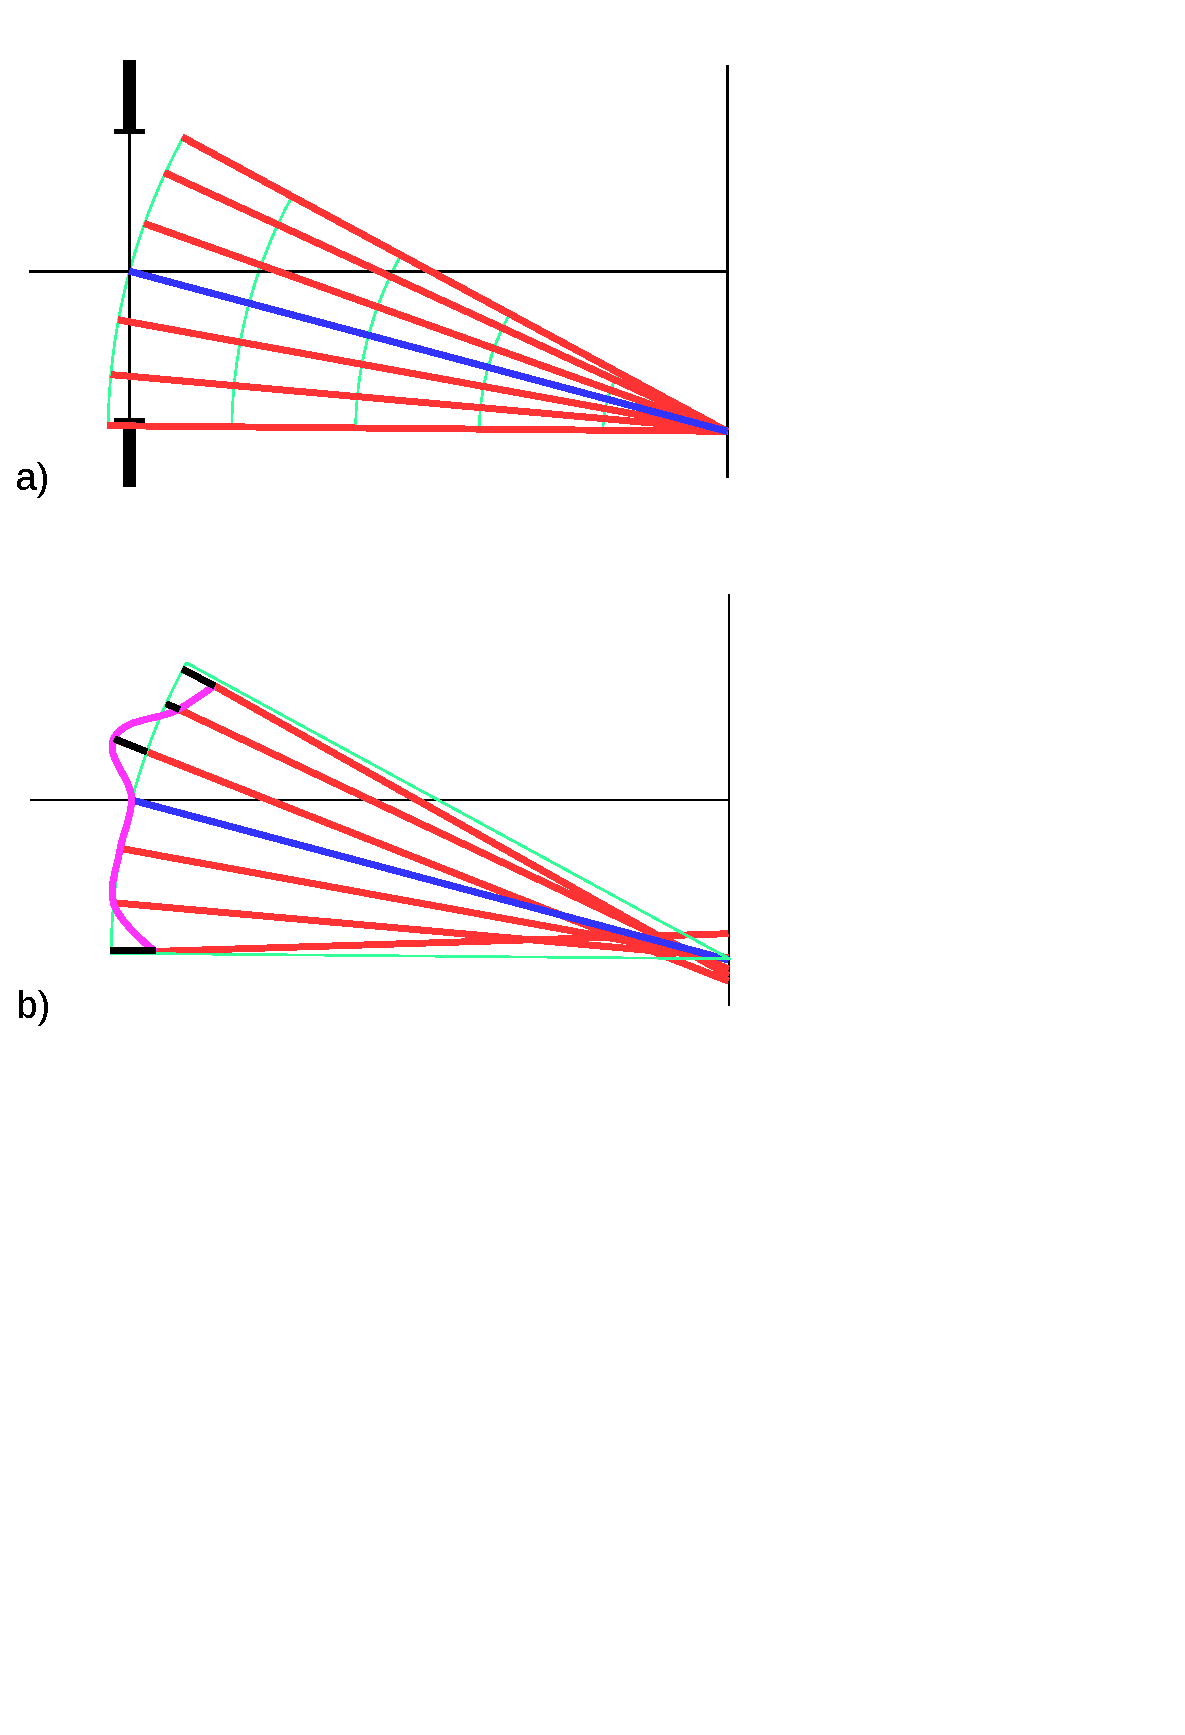
\includegraphics[width=0.5\columnwidth]{waveaberrations}
  \caption{a) In a perfect system, according to the Fermat principle, all rays have the same time of flight from the object to the image. b) In a real system, wave aberrations occur. A line of constant time of flight is displayed in magenta.
  Wave aberrations are the optical path differences corresponding to the difference in time of flight when hitting the exit pupil reference sphere.}
  \label{fig:waveaberrations}
\end{figure}

\subsection{Calculation of wave aberrations}
\remark{this only works for on axis field points}

Assume we know the position $x_{im}, y_{im}$ and direction $\Vector{d}$ of a set of rays in the image plane and their geometric path length from the object to the image.
To obtain the wave aberrations, we intersect the rays with the spherical exit pupil.
The task is similar to the intersections performed throughout the raytracing, see section \ref{subsection:spheres}.
We center our coordinate system around the chief ray image position.

\begin{eqnarray}
 \Location &=& \begin{pmatrix} x_0 \\ y_0 \\ 0 \end{pmatrix} + \Vector{d} t \\
 \Location^2 &=& R^2
\end{eqnarray}
with
 \begin{eqnarray}
 \begin{pmatrix} x_0 \\ y_0 \end{pmatrix} &=& \begin{pmatrix} x_{im} \\ y_{im} \end{pmatrix} - \begin{pmatrix} x_{chief,im} \\ y_{chief,im} \end{pmatrix} \\
 z_{im} &=& 0 \\
 | \Vector{d} | &=& 1
\end{eqnarray}
Here, $R$ is the distance between exit pupil and image, and $t$ is the geometric path length of the back-propagation.

We find
\begin{eqnarray}
 R^2 &=&  t^2 + 2 (d_x x_0 + d_y y_0) t + x_0^2 + y_0^2 \\
 t_{1,2} &=& - (d_x x_0 + d_y y_0) \pm \sqrt{ (d_x x_0 + d_y y_0)^2 - (x_0^2 + y_0^2) + R^2 }
\end{eqnarray}

We assume that the macroscopic distance between image and exit pupil $R^2$ term under the root is much larger than the microscopic aberrations and use a Taylor expansion
\begin{eqnarray}
 t_{1,2} &\approx& R - (d_x x_0 + d_y y_0) \pm 
 \left[ 
   \frac{1}{2R} \delta - \frac{1}{8R^3} \delta^2
 \right]
 \\
 \delta &=& (d_x x_0 + d_y y_0)^2 - x_0^2 - y_0^2
\end{eqnarray}

The geometric path length $t$ is inserted into the material dispersion to obtain the retardation between exit pupil and image. After that, this propagation length is subtracted from the optical path length from object to image.
Another subtraction of the chief ray value normalizes the result.
By didviding with the vacuum wavelength, we obtain the wave aberration in number of waves.


\bibliographystyle{unsrt}
\addcontentsline{toc}{chapter}{Bibliography}
\bibliography{pyrate}



\end{document}
